\RequirePackage[hyphens]{url}
\documentclass[11pt,titlepage,dvipsnames,table,xcdraw]{article}
\usepackage{strath-dissertation}
\usepackage{setspace}
\usepackage{pdfpages}


\usepackage{babel}
\usepackage{lipsum} % For demonstration only.

%--------------------------------
% Degree settings
%--------------------------------
\newcommand{\degreename}{Bachelor of Science}
\newcommand{\coursename}{CS408: Individual Project}
\newcommand{\deptname}{Computer and Information Sciences}

\begin{document}

%--------------------------------
% Title page.
%--------------------------------
\begin{titlepage}
\vspace*{5mm}
\titletext{Developing a Perimenopausal Symptom Tracker to Aid in Symptom Awareness and Identification of Perimenopause}
\authortext{Kiran Mahn}
\vspace{15mm}
\degreetext{\degreename}{\coursename}
\vspace{40mm}
\centredcrest
\vspace{5mm}
\depttext{\deptname}
\vspace{5mm}
\datetext{April, 2025}
\end{titlepage}

%--------------------------------
% Front matter numbering.
%--------------------------------
\pagenumbering{roman}
\setcounter{page}{2}

%--------------------------------
% Setting counter depth.
%--------------------------------
\setcounter{secnumdepth}{3}
\setcounter{tocdepth}{2}

%--------------------------------
% The front matter.
%--------------------------------
\setstretch{1.2} % 1.5 line spacing. 

%Abstract

%    Introduction
%    Background Literature
%    Specification & Design
%    Implementation
%    Evaluation
%    Results
%    Discussion & Reflection
%    Future Work
%    Conclusion

%References
%Appendices


\begin{abstract}

%% Susan: 
%% Update: fields.. advance - not advances
%% peri-menopausal > perimenopausal
%% learn > learning
%%
%% Suggest you rephrase future work as follows: 
%% The results of this study show that the app is usable and effective. 
%% Future work, that would also be helpful to perimenopausal women, includes  
%% a classification quiz to determine which stage of menopause the user is in, 
%% along with more detailed analysis of user data, and more learning resources.
As the fields of medical technology and digital health advances, more can be done to support peri-menopausal women through this life transition. Without proper education for doctors or the public, the everyday woman increasingly turns to technology to track her symptoms and take care of herself. However, FemTech corporations are using surveillance capitalism to sell these women's personal information which can have extremely serious ramifications for the women whose data is sold. During this study, research is done to determine the best way to help these women, and to develop a perimenopausal symptom tracking app that focuses on privacy and education. The app is designed to be user-friendly and intuitive, with a clean and simple design. The app has been evaluated using the System Usability Scale (SUS) and the Mobile App Rating Scale (MARS) to determine its usability and effectiveness. The app has been compared to other apps on the market to determine its strengths and weaknesses. The results of this study show that the app is usable and effective, but to be most helpful to perimenopausal women, a classification quiz to determine which stage of menopause the user is in should be added along with more detailed analysis of user data, and more learn resources.

\end{abstract}





%\section*{Declaration}
This dissertation is submitted in part fulfilment of the requirements for the degree of \degreename
in \coursename of the University of Strathclyde. 

I declare that this dissertation embodies the results of my own work and that it has been composed by myself. 

Following normal academic conventions, I have made due acknowledgement to the work of others. 

I declare that I have sought, and received, ethics approval via the Departmental Ethics Committee as appropriate to my research. 

I give permission to the University of Strathclyde, Department of \deptname, to provide copies of the dissertation, at cost, to those who may in the future request a copy of the dissertation for private study or research. 
and permit  Department of \deptname at the University of Strathclyde to place a copy of the dissertation in a publicly available archive. 

% Change this as needed,
(please tick) Yes [X] No [\quad] 

I declare that the page count for this dissertation (including title page, declaration, abstract, acknowledgements, table of contents, list of illustrations, and references  is XXX pages. % MUST BE 50 or LESS

I understand that project markers are not obliged to read any appendices I include in this dissertation.


I confirm that I wish this to be assessed as a Type 1 2 \circled{3}  Dissertation (please circle).

{\small 1=Software Development;
2=Experimentation-based with Significant Software Development;
3=Experiment-based.}


\begin{tabular}{|c|p{8cm}|}
\hline
 Signature:    &  \\ \hline
 Date:    & \\ \hline
\end{tabular}


%% Susan: 
%% Consider replacing the clearpage declaration below with a vspace
%% It'll save you a page, by putting introduction and acknowledgements
%% on the same page.
%% Use vspace like its used on the title page to add space between them.
\clearpage
\section*{Acknowledgements}

I would like to thank the participants who evaluated my project and my supervisor.






  % Uncomment to include this page.

%--------------------------------
% Tables of contents.
%--------------------------------
\setstretch{1.0} % 1.0 line spacing.  
\clearpage
\tableofcontents
%\listoffigures   % Uncomment for a list of figures.
%\listoftables    % Uncomment for a list of tables.
\clearpage

%--------------------------------
% The body of the document.
%--------------------------------
\pagenumbering{arabic} % Page numbering for rest of document.
\setstretch{1.5} % 1.5 line spacing. 
\section{Introduction}

The perimenopause is an ill-defined time period that surrounds the final years of a woman's reproductive life\cite{Santoro2016}. Perimenopause is a transitional phase that is not well understood by many individuals including doctors, leading to a lack of awareness and knowledge about the symptoms and management strategies. Due to this lack of education and awareness, many individuals do not realise that the psychological, hormonal, and physical changes they are experiencing are due to perimenopause, leading to confusion and frustration\cite{Muir2022}. There are many digital tools to support those currently in menopause, but there is a gap in the market for digital tools that support individuals who are entering the perimenopause phase of life. What makes these apps and tools useful to a perimenopausal women and what are the key features that are needed to support them during this time? This project aims to answer these questions by evaluating existing menopause apps, identifying areas for improvement (particularly in data privacy), and addressing them by creating a user-friendly and educational, and privacy-focused perimenopausal symptom tracking app.

After evaluating existing apps and identifying a gap in the market, this project moved into the design phase. A methodology was established for managing the project, and processes were designed for collecting user requirements for the symptom tracker app. Additionally, a framework for app testing was created to evaluate usability. Both functional and non-functional requirements were identified, and the app’s frontend interface and backend system for data management were designed.  

During the implementation phase, the user interface was prototyped, app features were developed using reusable widgets, file management was integrated, and thorough testing was conducted. To ensure quality, multiple rounds of evaluation were carried out with users. These evaluations verified that the app meets its goals, fulfills the needs of its target audience, and remains competitive with existing apps in the market. % Add one file per section.
\clearpage
\section{Background Literature}\label{backg}

\subsection{Perimenopause}
The American Journal of Epidemiology\cite{Brambilla1994} states that perimenopause is the transition period of a womans life, which starts with a natural shift in ovulation and menstruation patterns and/or increased symptoms, and ends when a woman enters menopause. It classifies menopause as when a woman has not had her period for a year. This Lancashire and South Cumbria NHS Foundation Trust's article on Perimenopause, Menopause, and Pain\cite{LSCFT2024} states that during perimenopause, the body's production of estrogen, testosterone, and progesterone fluctuates significantly and can stay low forever if no treatment is taken. This change in hormones drastically changes the way a woman's body and mind work. A Swiss Perimenopause study\cite{Willi2021} found that women experiencing lower estrogen and progesterone levels had higher suicide intent scores and were more likely to develop depression, which is backed up by another study from the Journal of Psychiatric Research which found a correlation between low progesterone states and suicide\cite{BACAGARCIA2010209}. Other effects of perimenopause are much more common, and perimenopause may not be the obvious source. During Perimenopause, 80\% of women experience hot flashes\cite{Bansal2019}, 77\% joint pain\cite{ScienceDaily2013}, 60\% memory issues\cite{Gaytri2018}, over 20\% experience heart palpitations\cite{Sheng2021}, 1/4 women have really heavy periods\cite{Harlow2011}, 50\% of women say it negatively impacts their sex lives\cite{BMS2016}, and 1/10 women leave their jobs because of menopausal symptoms\cite{Brewis2017}. It therefore comes as no surprise that almost 90\% of women seek out their healthcare provider for advice on how to cope\cite{Guthrie2003}. However, in the US, 3/4 of women who ask for medical help are left untreated, causing women to turn to other sources of help and information\cite{Wolff2018}. 

\subsection{Menopause Education}
A University College London publication on women's post reproductive health\cite{Aljumah2023} explores the extent of knowledge women have about menopause. When it comes to menopause, most women are left untreated and unsupported. Without sufficient education, most are left suffering due to hormonal imbalance and lifestyle changes they are unprepared for and do not have the information they need to help them cope. In this study of 829 postmenopausal women, 90\% were never educated about the menopause. It is rarely included in sexual education received in school, and though awareness is increasing, it is still rarely talked about in the media and considered a taboo and private subject only to be talked about with your doctor\cite{Muir2022}. Talking to the doctor is also problematic as doctors are also not well educated on menopause\cite{MenopauseSupport2021}. The NHS site on the treatment of menopause\cite{NHS2022} states that many menopause symptoms can be effectively treated with hormone replacement therapy (HRT), even symptoms such as hot flushes can improve within a few weeks. However, a study of 3000 british menopausal women who complained to their doctors of low mood or anxiety symptoms found that 66\% were offered anti-depresseants instead of hormones\cite{NewsonHealth2019}. In fact, 1/4 of women are on anti-depresseants post menopause\cite{Brody2020} despite the fact that antidepressants don't help low mood in menopausal women with hormone imbalances, and according to the National Institute for Health and Care Excellence\cite{NICE2019} HRT should be offered first. This may be largely due to lack of education doctors receive about menopause. 41\% of UK medical schools do not give any mandatory menopause education\cite{MenopauseSupport2021}. Professor Joyce Harper, an internationally renowned, award-winning scientist and a professor of reproductive science at UCL, states that “The data shows that women have a lack of education about this key life stage. Together with a reported lack of education from their healthcare professionals, women may be left undiagnosed and unsupported”\cite{UCL2023}.

\subsection{Symptom Tracking Apps and Technology}
When women do not receive education from school, their communities, or their doctors about peri-menopause, they will look for tools and education from other sources such as websites or apps to research, track, and analyse their experience. Over 50 million women worldwide use apps to track their menstrual cycle and examine a variety of other cycle-related factors\cite{Kelly2023}. There are 300 menstrual tracking applications available for download and an estimated 200 million downloads worldwide\cite{Eschler2019}. Symptom monitoring and appraisal methods are effective for reducing menopausal symptoms, and improving health awareness, shared decision-making, patient-doctor communication, and treatment goal setting\cite{Andrews2021}. 

While these apps can be effective tools for dealing with symptoms, one of the most prominent issues with these apps is the lack of privacy. The apps often earn profits by selling users’ data to third parties, even if there is a promise of privacy advertised by the companies\cite{Gilman2021}. An article by the Director of Research for Sexual and Reproductive Health and Rights, Population Institute in Washington, DC titled, “Missed period? The significance of period-tracking applications in a post-Roe America” highlights the increased concerns around this surveillance capitalism since the June 2022 overturning of Roe vs Wade in the US stated that the right to abortion is not constitutionally protected\cite{CoenSanchez2022}. It further explores how users personal tracking data may be used against them in court as evidence of having an abortion regardless of miscarriages, irregularities in menstrual cycles, and/or imperfect engagement with a period-tracking app. Some apps have even gone on record to say they will hand over users data to law enforcement if asked. The article even explains how some experts advise people who menstruate to track their periods on paper as opposed to using an app for their own protection. These `FemTech' mobile apps currently fall outside of the scope of the Health Insurance Portability and Accountability Act, which protects sensitive health information from being disclosed by covered entities without the patient’s consent or knowledge\cite{OCR2022}. This highlights the ever increasing need for privacy in menstrual tracking apps. 

A study\cite{Chan2019} exploring the design experience of digital period trackers found that to best design digital period trackers for users, Hertzum’s images of universal, situational and cultural usability should be used. This correlates with Dawsons concepts of evidence-based, usable, readable, interactive, and culturally sensitive design choices for health apps \cite{Dawson2020}. It found that a good period tracking app should know the users life stage, medical “situation”, contraception, purpose of tracking, and tracking interests. It also highlights the need for education resources within these health apps and the importance of users having access to relevant, reliable health information such as including external links to information. 

Not only do these peri-menopause apps have to be free, private, and personalised, but they must be accessible to all who want to use them. The European Accessibility Act (EAA) becomes law on the 28th of June 2025. The EAA is a landmark legal change that will improve the lives of disabled people by ensuring equal access to digital products and services for European Union (EU) consumers\cite{AbilityNet2024}. The EAA requires products and services to be Perceivable, Operable, Understandable, and Robust (known as POUR). 

So given these issues, this project attempts to address them by developing an app which allows women to track, analyse, and learn about peri-menopause while ensuring a focus on users privacy and anonymity. 
 % Add one file per section.
\clearpage

\section{Specification \& Design}\label{process}

Before beginning the process of gathering user requirements, an ethics form must be completed to ensure that the research follows ethical guidelines. To better understand user needs, a User Requirements survey was designed. In preparation, research was conducted through books on women’s experiences during perimenopause, including works by Kat Muir\cite{Muir2022} and Davina McCall\cite{McCall2022}, as well as reviewing research papers on health-tracking applications and a review of existing apps on the market to assess current solutions. Privacy emerged as a significant concern, with many apps engaging in surveillance capitalism and selling user data, often without informing or misleading the user\cite{Gilman_2021}\cite{FTC2021}. Hackers are lured to health data such as that stored by symptom tracking apps beacuse on the black market, a persons medical data sells for 50 times what credit card information sells for\cite{Rosato2020}. To ensure a user-centered approach, User Stories were developed to capture potential users’ needs and expectations. As the project developed, user requirements and stories were continually adjusted to best reflect the goal of this project. The Design Testing Stage incorporates the System Usability Scale (SUS) evaluations and A/B Testing through microsoft forms. User interviews are also conducted to refine the design based on feedback. Recruitment for testing was also planned, stating the target audience for this study was women between the ages of 30 and 65.


\begin{table}[h!!]
  \caption{User Requirements Survey Results}
  \resizebox{\textwidth}{!}{
      \begin{tabular}{lll}
      \hline
      User Requirements Survey Results (n = 11)                                       &                        &      \\ \hline
      What stage of menopause are you in?                                             & Premenopausal          & 9\%  \\
                                                                                      & PeriMenopausal         & 55\% \\
                                                                                      & Menopausal             & 0\%  \\
                                                                                      & PostMenopausal         & 18\% \\
                                                                                      & Other                  & 18\% \\
      Do you experience any Period, Perimenopause, or Menopause symptoms?             & Yes                    & 82\% \\
                                                                                      & No                     & 18\% \\
      What peri-menopausal / menopausal symptoms do you currently experience, if any? & Hot Flashes            & 9\%  \\
                                                                                      & Mood Swings            & 13\% \\
                                                                                      & Irregular Periods      & 4\%  \\
                                                                                      & Sleep Problems         & 13\% \\
                                                                                      & Joint and Muscle Aches & 16\% \\
                                                                                      & Vaginal Dryness        & 13\% \\
                                                                                      & Night Sweats           & 6\%  \\
                                                                                      & Have to pee often      & 9\%  \\
                                                                                      & Other                  & 9\%  \\
      How do you track your symptoms or periods?                                      & Smartwatch             & 18\% \\
                                                                                      & Manually recorded      & 36\% \\
                                                                                      & No tracking            & 18\% \\ \hline
      \end{tabular}
  }
\end{table}

\subsection{Methodology}
Following research on the different available software lifecycle approach softwares and methods available, Kanban boards were chosen as they are easy to maintain for one person, help with workflow, and have been proven to work in a student setting as mentioned prior. GitLab Issue boards were selected as the platform to host the Kanban as each issue card can be linked to branches within repositories to keep track of which tasks and changes are for which branches to improve organisation. Three labels: Code, Writing and research, and Critical, were also added to signify the type of task for each issue card. The Kanban board included four sections, one for each label and one for closed tasks. Gitlab would automatically sort each task into the relevent section based on its labels. The board was updated regularly to reflect the current status of each task, and tasks were moved from one section to another as they were completed. This resulted in tasks that were easy to priortiise, order, track, and complete on time. See Figure 1 for the Kanban board.

\begin{figure}[h!!]
  \begin{center}
    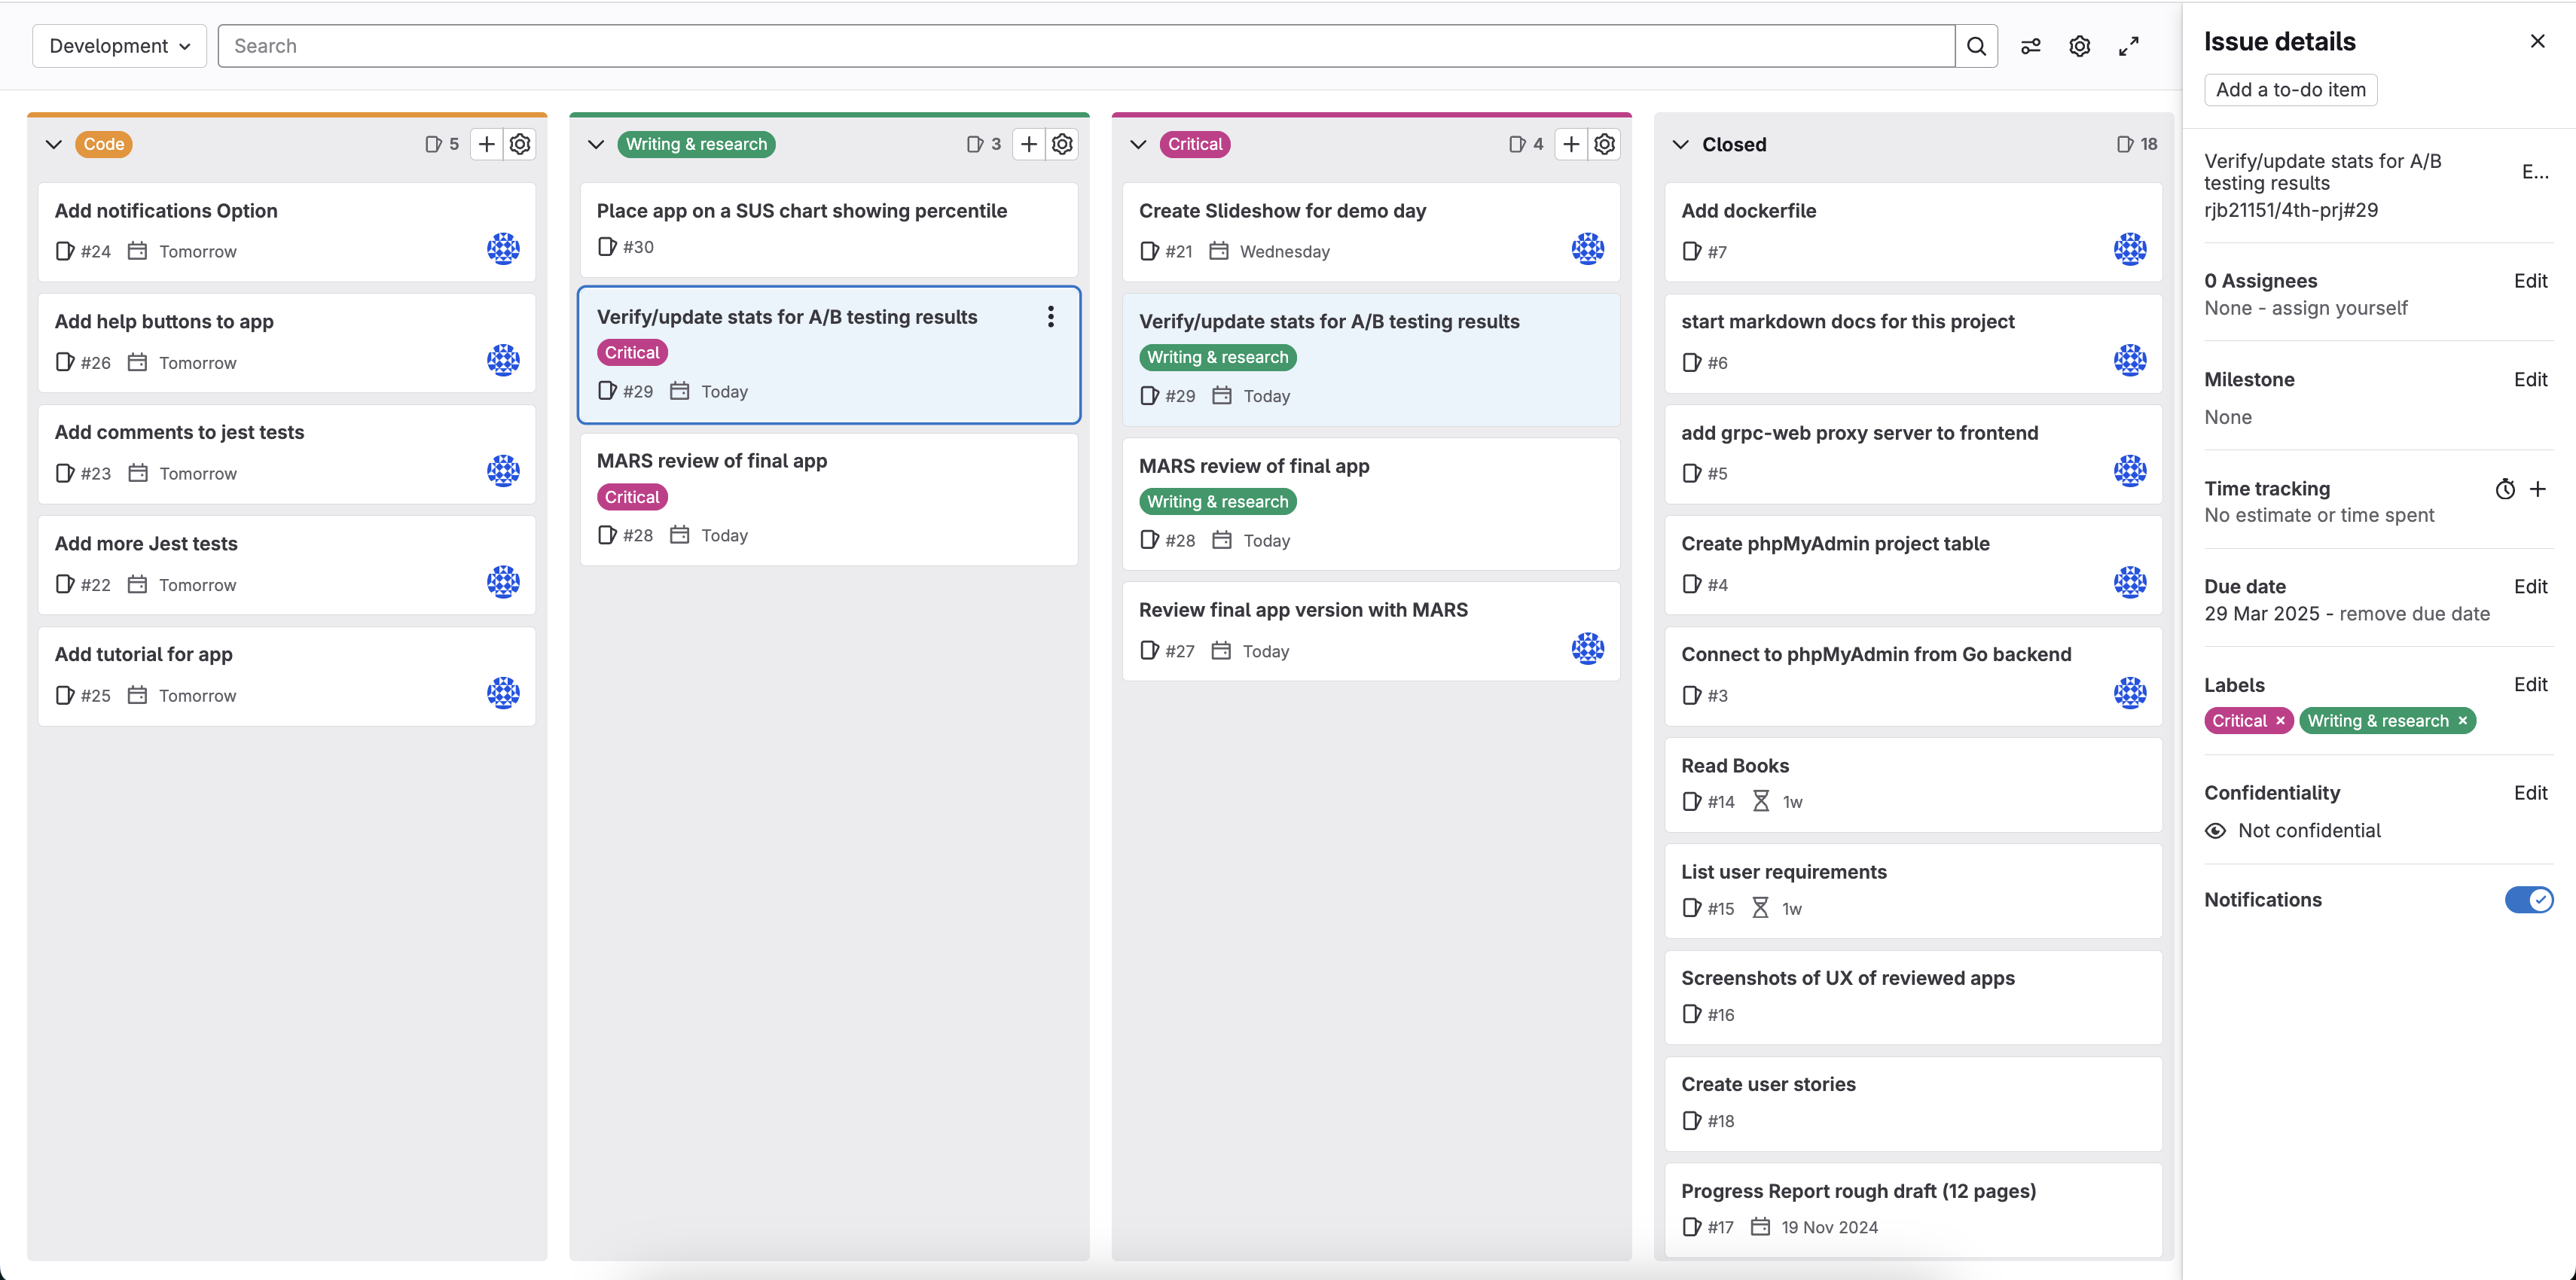
\includegraphics[scale=0.25]{Kanban.png}
    \caption{Kanban board on GitLab.}
    \label{figure:kanban-board}
  \end{center}
\end{figure}

Around after a month of progress, a network diagram was made to find the critical path in order to correctly prioritise work. Once a list of the main activities was made, the dependencies of each activity were identified and the time it would take to complete each activity was estimated. The critical path was then identified by finding the path through the network diagram with a float or lewway of zero. The critical path is the sequence of activities that must be completed on time for the project to be completed on schedule. The critical path is important because it helps to identify which activities are most important for the success of the project and which activities can be delayed without affecting the overall project timeline. See Figure 1 for the network diagram. The critical path activities are highlighted in red. From the network diagram, it was concluded that writing the report and obtaining feedback was the most important aspect of this project and should be prioritised over other tasks. The network diagram also helped to identify potential bottlenecks in the project timeline and allowed for better planning and scheduling of tasks.

\begin{figure}[h!!]
  \begin{center}
    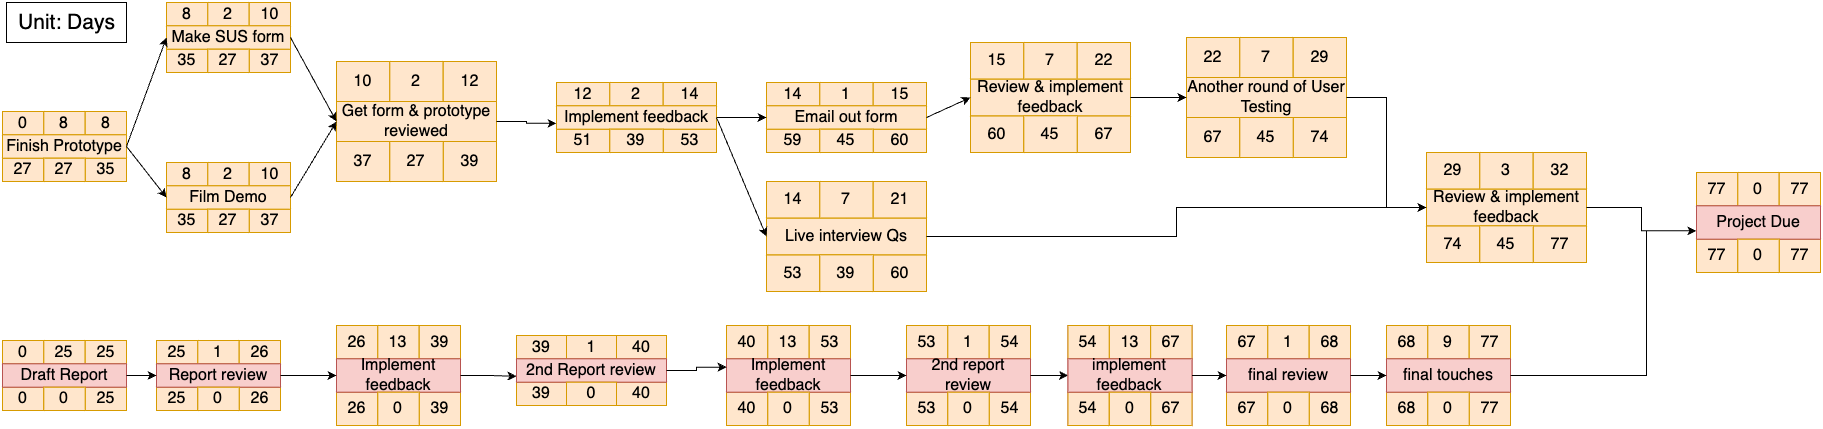
\includegraphics[scale=0.2]{NetworkDiagram.drawio.png}
    \caption{Network Diagram showing critical path.}
    \label{figure:network-diagram}
  \end{center}
\end{figure}
 
\subsection{Analysis}
Given many peri-menopausal women are not receiving support from the government education system or their doctors\cite{Aljumah2023}\cite{MenopauseSupport2021}\cite{UCL2023}, additional resources and tools must be provided to help them navigate this stage of life. With the rise of technology, several tools are now available to allow women to track their peri-menopausal symptoms. However, these tools are often not user-friendly, do not provide enough educational information, or are not privacy-focused. The issue around privacy is especially concerning as many apps are selling user data to third parties without user knowledge and consent, and in today's political climate this can result in the incarceration of the user in some parts of the US\cite{Kelly2023}. Since there are no apps that provide a comprehensive solution to these problems, the goal of this project is to create a user-friendly, educational, and privacy-focused peri-menopausal symptom tracking app.

\subsection{Requirements}

\subsubsection{Functional Requirements}
This Apps functional requirements were prioritized based on user needs and the project goal. Essential functional requirements impacting usability such as being able to navigate to a screen were prioritised over design and content details. The following functional requirements were identified:

\begin{itemize}
      \item Users must be able to log their period start and end dates to track cycle and period length.
      \item Users must be able to log their peri-menopausal symptoms and their severity daily to track changes over time.
      \item Users must be able to edit or delete logged symptoms and period data at any time.
      \item The app must store all user data locally using AsyncStorage on the users device, ensuring no data is stored on external servers.
      \item The app must include a calendar view where users can see logged symptoms and period data over time.
      \item The app must provide an option to reset user data to align with privacy-focused design principles
      \item The app must provide graph-based visualizations showing symptom frequency and period heaviness trends over time.
      \item The app must calculate and display the most common symptom based on user entries.
      \item The app must provide cycle length insights based on logged period data.
      \item The app must calculate average period length based on tracked cycles.
      \item Users must be able to access an Analysis Tab summarizing trends.
      \item The app must feature a Learn Page with information on perimenopause and related topics.
      \item Users must be able to access external links to trusted resources for more detailed information.
      \item The app must follow EU accessibility standards, including text scaling, color contrast, and screen reader compatibility.
      \item The app must support multiple languages to accommodate diverse users.
      \item Users must be able to enable or disable notifications/reminders for period tracking or symptom logging.
      \item The app must work fully offline, allowing users to track symptoms and view their data without an internet connection.
      \item The app must not crash or freeze during normal usage.
\end{itemize}

\subsubsection{Non-Functional Requirements}
\begin{itemize}
  \item The app should be easy to use and navigate, with a clean and simple design.
  \item The app home page should load within 3 seconds.
  \item All data visualization such as graphs, calendar, and analysis charts should render in under 2 seconds.
  \item The app should allow easy localization to support multiple languages.
  \item The UI should offer a dark mode and high-contrast mode to improve readability for all users.
  \item All text elements must support dynamic font resizing based on user preferences.
  \item The app should look the same for various screen sizes, including tablets and smaller phones.
  \item The app must be designed with easy language switching to support multiple languages in the future.
  \item The app should maintain consistent navigation and UI patterns across all features to reduce confusion.
\end{itemize}

\subsection{Design}

\subsubsection{Interface Design}
At the beginning of the design process, low fidelity wireframes were created using Figma. See Figure 1.

\begin{figure}[h!!]
  \begin{center}
    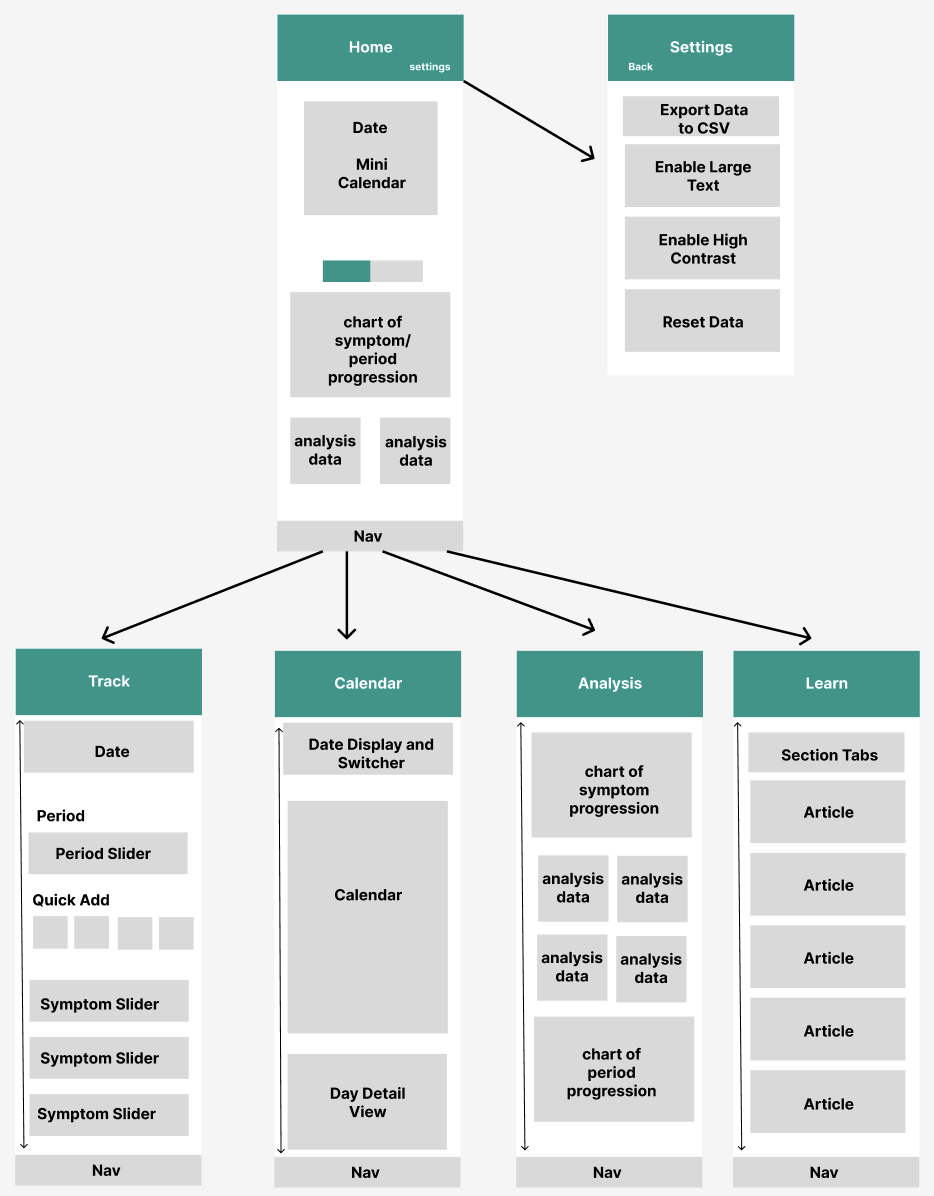
\includegraphics[scale=0.7]{Figma-1.png}
    \caption{Wireframe of App on Figma.}
    \label{figure:figma-1}
  \end{center}
\end{figure}

The color scheme was chosen to be relaxing and calming  through the use of blue and green tones. The app was designed to be user-friendly and intuitive, with a focus on simplicity and ease of use. The design was also created with the goal of making it easy for users to navigate the app and find the information they need, as well as be responsive and work well on different screen sizes, including tablets and smaller phones.  

The design was then fleshed out into a more detailed figma design. See Figure 2.

\begin{figure}[h!!]
  \begin{center}
    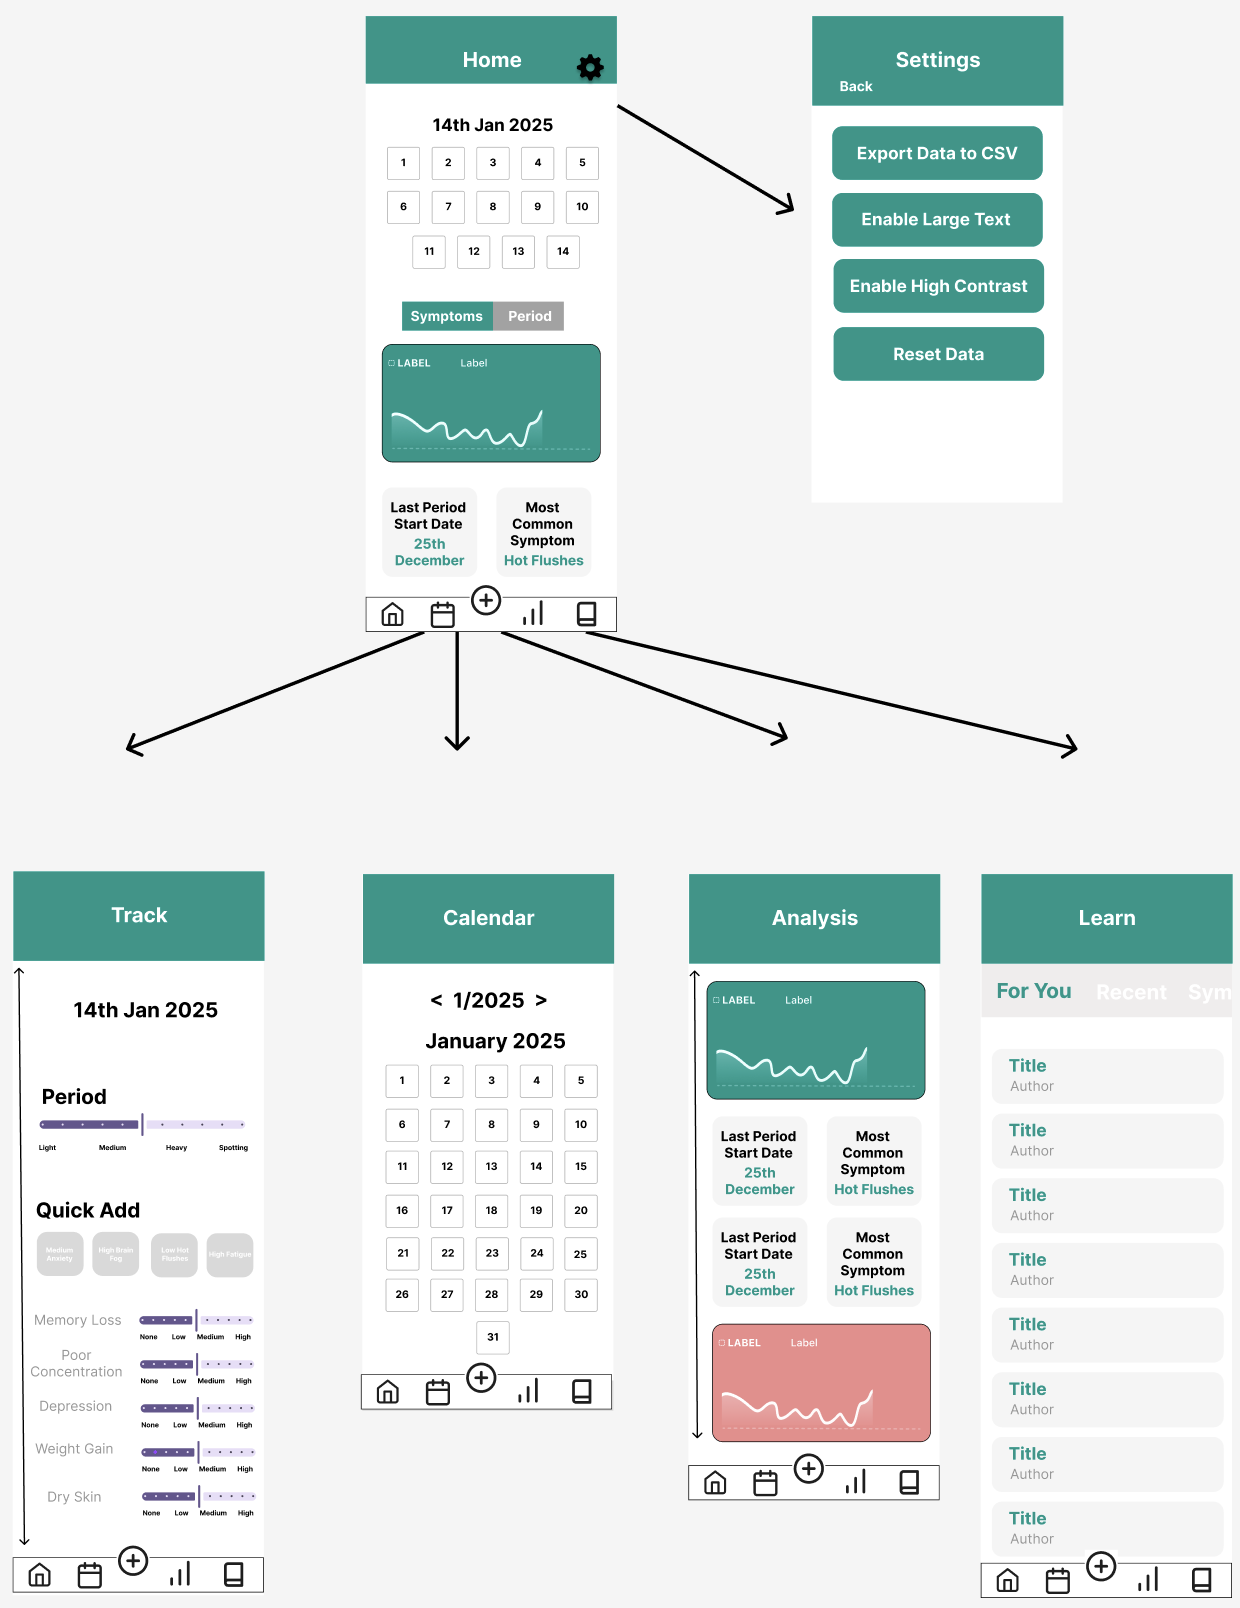
\includegraphics[scale=0.6]{Figma-2.png}
    \caption{Deatiled Draft of App on Figma.}
    \label{figure:figma-2}
  \end{center}
\end{figure}

The design was created with a focus on simplicity and ease of use. The app was designed to be user-friendly and intuitive, with a clean and simple design. The final color scheme was chosen to be calming and easy on the eyes, with a focus on blues and greens. Feedback from user evaluations was incorporated into the design to ensure that it met the needs of the target audience. Some user feedback that was implemented includes adding days of the week to the mini calendar in the home page, making the track button in the nav bar larger and a different color to make it more visible, ability to refresh the home page, and ability to track by clicking a day in the calendar. 

\begin{figure}[h!!]
  \begin{center}
    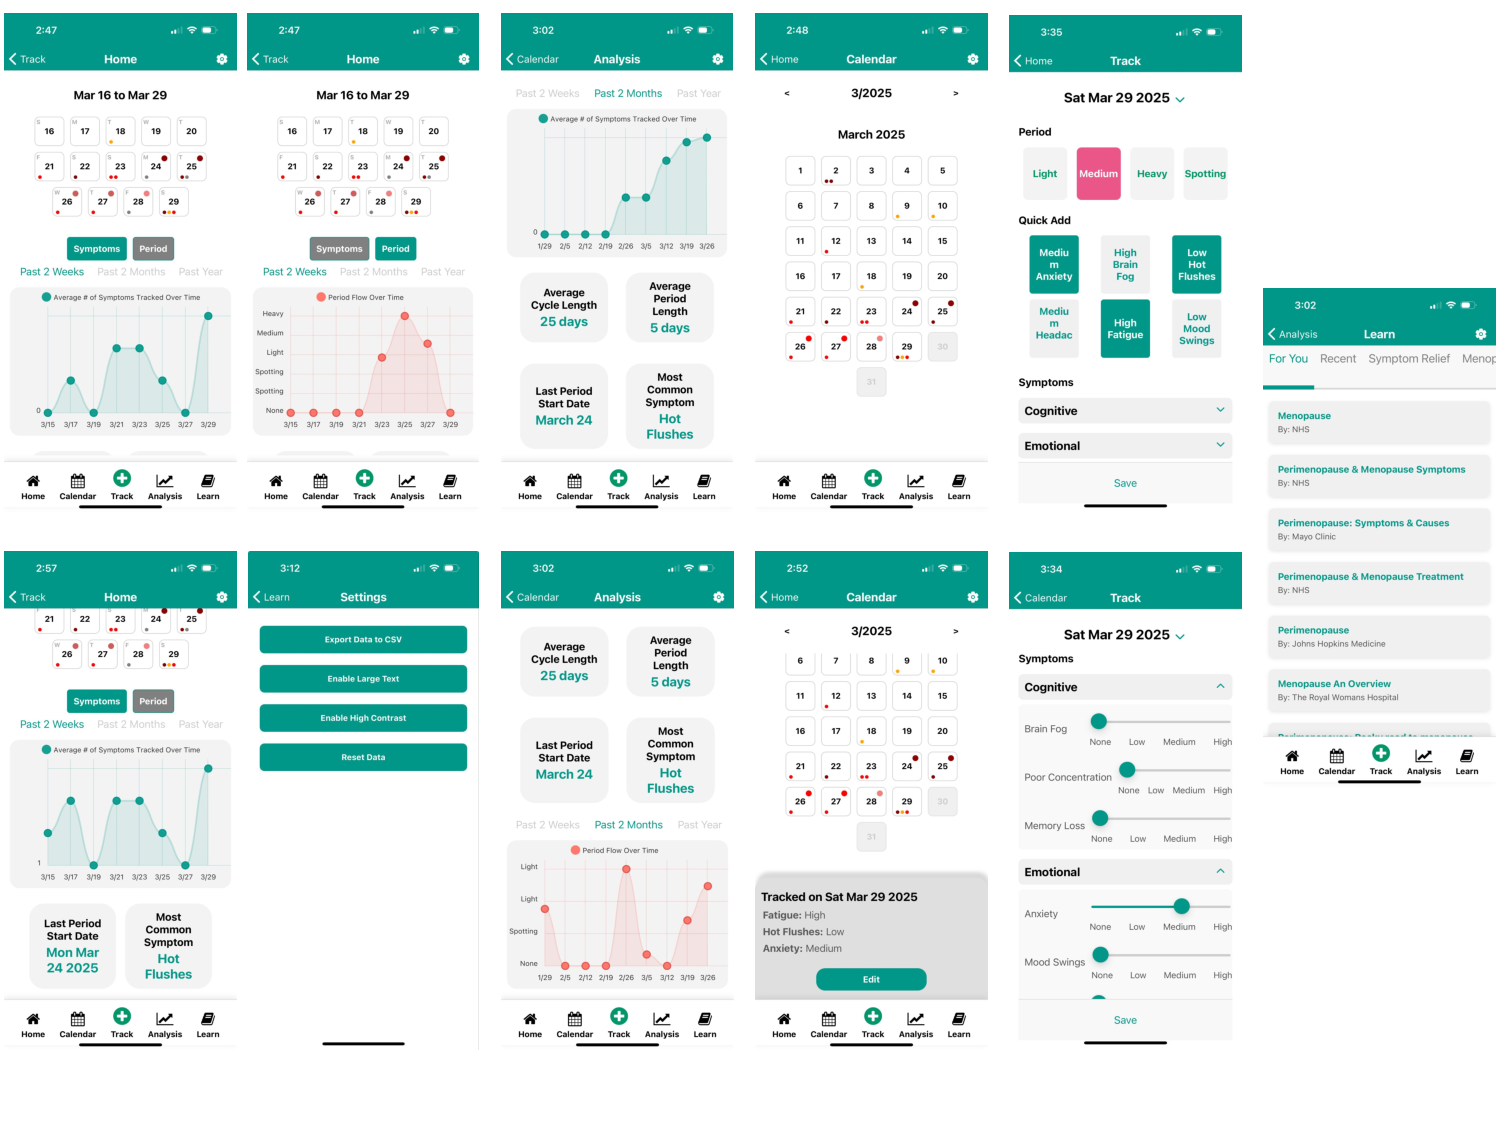
\includegraphics[scale=0.6]{app.pdf}
    \caption{Final React Native App Design.}
    \label{figure:app}
  \end{center}
\end{figure}


The app was then compared to the EU WAG 2.1 accessibility standards and adjusted to be accessible to all users, with large text and color contrast options in the settings. Figre 4 shows the app in dark mode with high contrast and large text mode enabled.
 
\begin{figure}[h!!]
  \begin{center}
    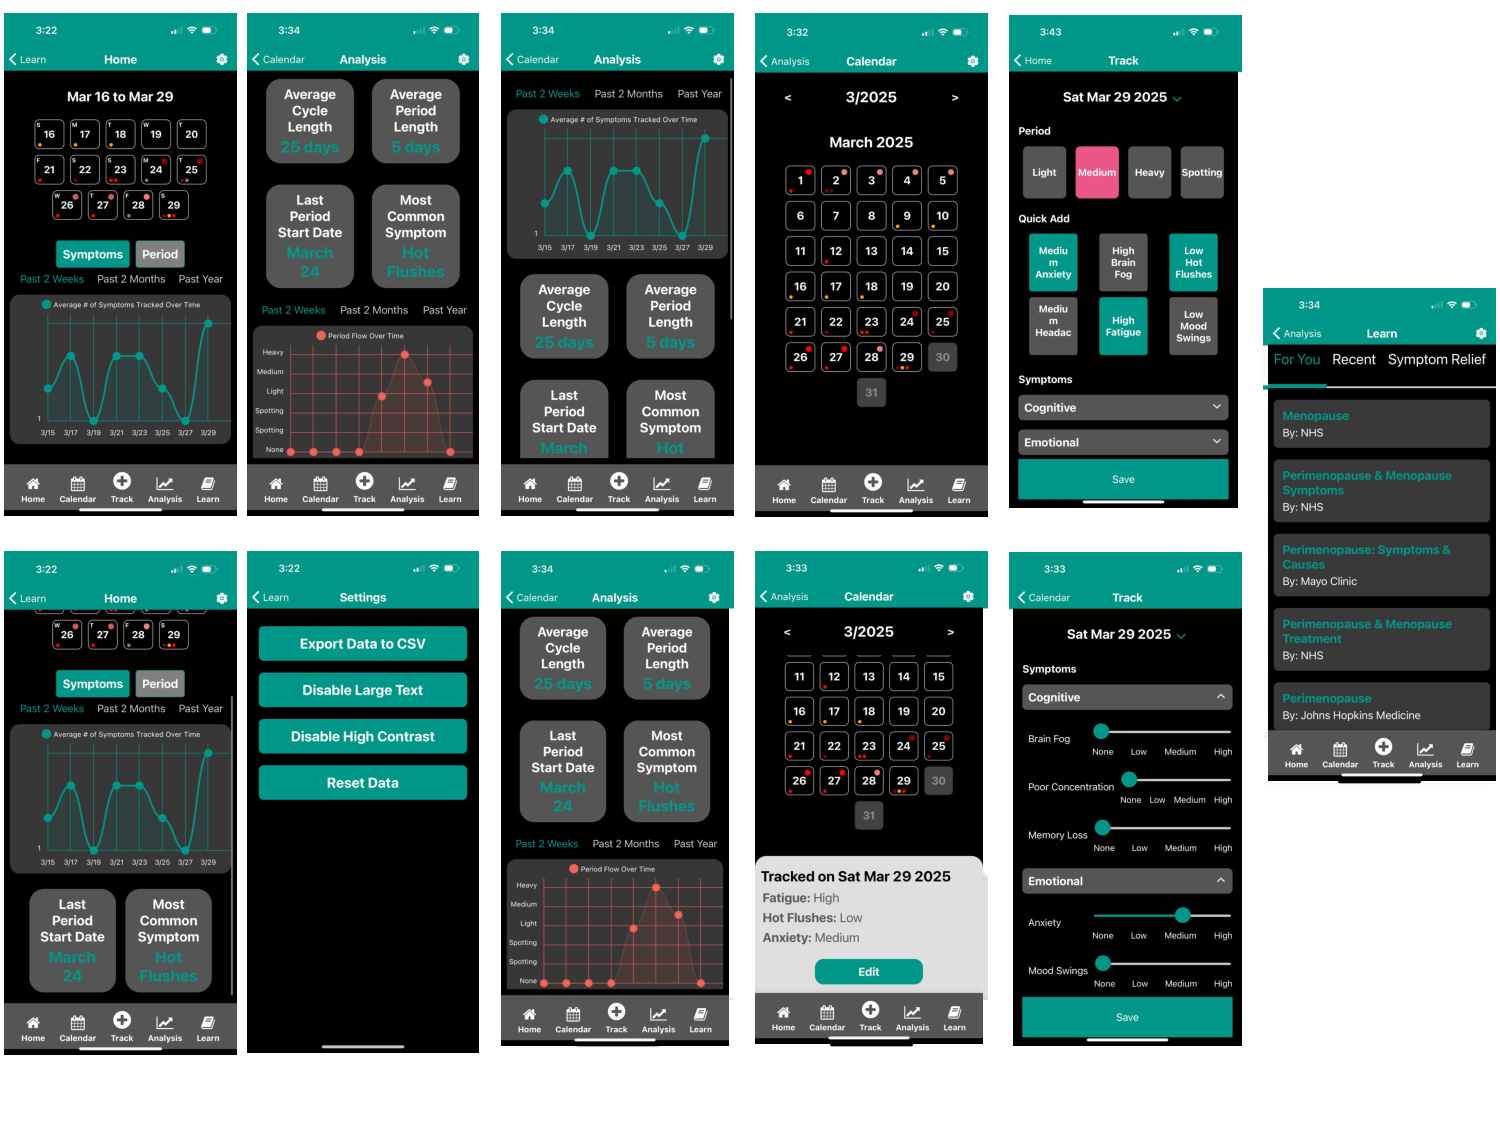
\includegraphics[scale=0.6]{app-Accessible.pdf}
    \caption{Final React Native App Design with high contrast and large text on.}
    \label{figure:app-Accessible}
  \end{center}
\end{figure}

\subsubsection{System Design}
In the interest of protecting user privacy, there is no database and all data is stored on the user's local device. The data that is saved in AsyncStorage on their device is formatted as featured in the table below.

  \begin{table}[h!!]
    \caption{Structure User Data is Stored in AsyncStorage}
    \label{table:user-data}
    \begin{tabular}{llll}
    \hline
    Anonymous User &        &          &          \\ \hline
                  & Date1  &          &          \\
                  &        & Symptom1 & Severity \\
                  &        & Symptom2 & Severity \\
                  & Date2  &          &          \\
                  &        & Symptom1 & Severity \\
                  &        & Symptom2 & Severity \\
                  & Date n &          &          \\
                  &        & Symptom1 & Severity \\
                  &        & Symptom2 & Severity \\ \hline
    \end{tabular}
    \end{table} % Add one file per section.
\clearpage
\section{Product}\label{product}

\subsection{Implementation}

\subsubsection{Prototyping}
During the design and initial development phase, a prototype was made using React and js with an npm node.js server. The change to another solution was much needed as using React with localstorage or a database comes with many privacy and security concerns that don't align with the functional requirements. The next Implementation was using Go and React with typescript for more security but due to typescript being a more strict language development was significantly slowed down along with the complexities of safely sending data back and forth between Go and React tsx. A GoLang Envoy Proxy was considered but due to the exponentially increasing complexity another solution was needed. 

\subsubsection{Expo \& React Native}
That is when the final implementation was decided to be a React native app that uses both typescript and javascript. This allowed for a lot of work to be moved over without rewriting files, as well as having the ability to use typescripts strict type checking for more complex files to make debugging easier and faster through type safety and reduces runtime errors. Expo was used for the react native app due to its easy routing capabilities, intuitive and easy testing setups, and debuggers. Nicola Corti who is on the React Native team at Meta said at the 2024 React keynote conference, \"Expo today, is the fastest way to bring your apps from idea, to production\". With Expo, code was transferred from the prototypes to a working React Native IOS Expo app that could be tested on iPhone in less than a day. Not only is it fast a react Native setup allows the use of AsyncStorage where the user data is safely stored on their device. This allowed user data to be stored without a username or password or any other identifiable details making the app completely anonymous. 

\subsubsection{The new React Native}
This app uses React Native 0.76.0, which is the latest version of React Native at the time of writing and has been in the works since 2018. This version includes many new features and improvements. The old react native used a bridge to asynchronouslt pass messages between the apps javascript and native code for IOS and Android, the new react native uses a JavaScript Interface (JSI) which allows direct method calls without the overhead of serializing data which greately improves efficiency\cite{ReactNative2024}. The new react native supports concurrent rendering which means the UI of the app looks smoother when applying updates. This new version of react native is enabled in this project and made development and the user experience much more enjoyable.

\begin{figure}[h!!]
    \begin{center}
      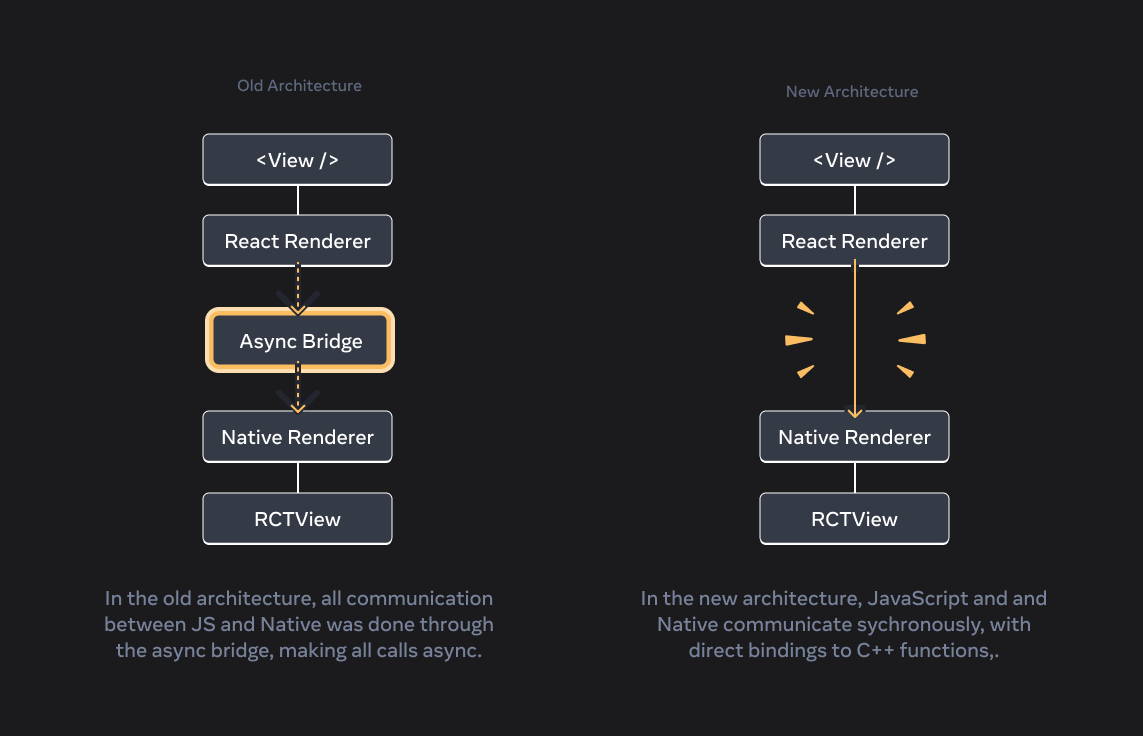
\includegraphics[scale=0.2]{react-native.png}
      \caption{The old and new React Native\cite{ReactNative2024}}
      \label{figure:react-native}
    \end{center}
  \end{figure}

\subsubsection{React Navigation}
In order to hand navigation within the app, React Navigation was used. React Navigation is a completely customisable routing and navigation library that works with React Native. The library supports both stack and tab navigation, making it easy to create a variety of navigation patterns such as the nav bar at the bottom of the app, and handling page switching via buttons in the app such as pressing on a calendar day box or a back button. 

\subsubsection{Wigits}
This app had many reusable components throughout the app. These components are called widgets and are used to create a consistent look and feel across the app while making the code easier to read and understand. The widgets are also used to create a consistent user experience, making it easy for users to navigate the app and find the information they need. Another pro of using widgets is that they can be easily tested and debugged, making it easier to identify and fix any issues that arise. Changing the wigit definition in one place will change the look and feel of the app in all places where the widget is used making the code easier to change, update, and understand for future developers. 

\subsubsection{Chart Kit}
Given many Doctors and women lack knoledge about perimenopause and the symptoms, the app uses a data analysis library called react-native-chart-kit to display the data in a visual way. This library is used to create charts and graphs that help users understand their data and identify patterns. The library supports a variety of chart types, including line charts, bar charts, and pie charts, making it easy to create a variety of visualizations. 

Two charts were created for the app: a symptom chart and a period chart. Since perimenopause is the time in a womans life when their period beins to change, the period chart is used to show the users period cycle and how it changes over time. This way, when a user bleeds inconsistenly or has a missed period, they can see how their cycle has changed over time and if it is normal for them. This data can then be exported to a csv file and shared with their doctor who can provide them with their expect opinion based on the users data. The period chart has three options, view data for the past two weeks, two months, or the past year. An algorithm was implemented that averages the data over time so it displays in an aesthetically pleasing way for the user. When two weeks is selected, data from every two days is averaged and showed on the chart. When two months is selected, data from every 7 days is averaged and showed on the chart. When a year is selected, data from every month is averaged and shown on the chart. Likewise, the Symptom chart averages the number of symptoms tracked over time and displays it on the chart. 

\subsubsection{Data Analysis}
To further support women in perimenopause, the analysis page in the app displays data that is relevant to a perimenopausal woman. This includes data commonly asked by a doctor such as the last period start date, average cycle length, most common symptoms, and average period length. The average cycle length is found by calculating the average number of days between the start of each period. The most common symptoms are found by counting the number of times each symptom is tracked and displaying the one with the highest count. The average period length is found by calculating the average number of days between the start and end of each period. This data is displayed in wigits, making it easy for users to understand, and easily accessible to share with their doctor.

\subsubsection{Settings Context}
As women enter perimenopause, they may experience symptoms such as brain fog, poor concentration, memory loss, dry eyes, blurred vision, and increased sensitivity to light. To help users manage their symptoms, the app includes a settings page that allows users to change the font size and color contrast of the app. This is done using a context provider that stores the user's settings in Async Storage. A settings-context typescript file was created that specifys the context type and the types of settings that the user can change which were specified as two booleans, one for large text and one for high contrast. It creates a context provider that wraps the app (used in layout.tsx) and passes the state of the users settings and a function to update the settings, making it easy to access the settings from within each component. These components have been written to dynamically change depending on the setting using in line css. 

\subsubsection{Expo FileSystem}
In order for users to export their data to a csv, expo FileSystem was used. This allows the app to create a file on the users device that can be opened in a spreadsheet program. FileSystem provides an API for accessing the file system, making it easy to work with files in a cross-platform way. The library also provides support for reading and writing files in different formats, such as JSON and CSV, making it easy to work with the users JSON data stored in Async Storage.

\begin{figure}[h!!]
    \begin{center}
      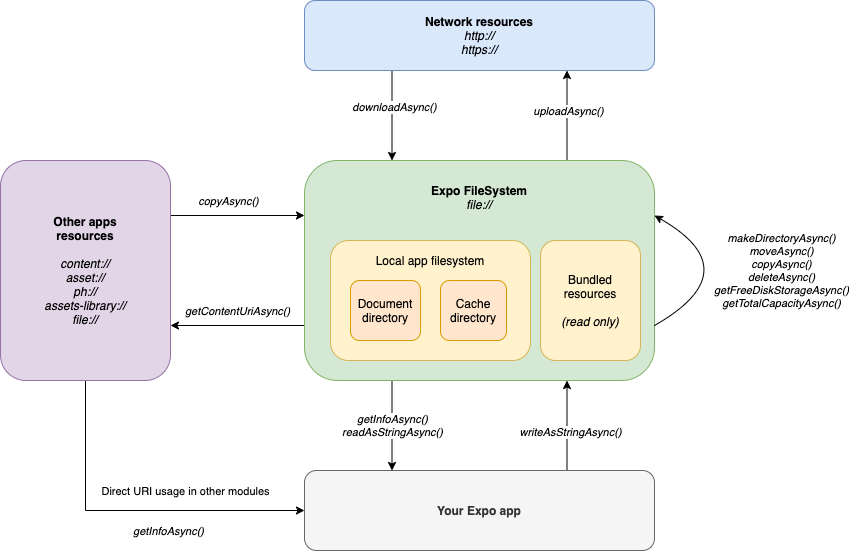
\includegraphics[scale=0.3]{file-system-diagram.png}
      \caption{The Expo File System\cite{ExpoFileSystem2025}}
      \label{figure:file-system-diagram}
    \end{center}
  \end{figure}

In order to implement FileSystem, the expo-file-system library was integrated into the app. When the user selects the export data to CSV button in settings, their data is fetched from Async Storage. Rows are defined for the CSV file for date, user, key, and value. Each object in the user data is iterated over to check if there is any null or empty data before adding the data to the CSV file using writeAsStringAsync(). The data is then shared with the user using shareAsync() which allows the user to specify where to store the file.

\subsection{Verification \& Validation}
Using Expo, the app was trialed and tested on mobile devices and emulators to ensure that the app was functioning as expected. The app was tested on iOS devices with different screen sizes to ensure that it was responsive and that the UI was consistent across all devices. The app was also tested for performance, and adjustments were made to ensure that it was fast and responsive by using a timer to measure the time it takes for the app and its different pages to load on click, comforming with the non-functional requirements. 

\subsubsection{Testing with Jest}

\begin{figure}[h!!]
    \begin{center}
      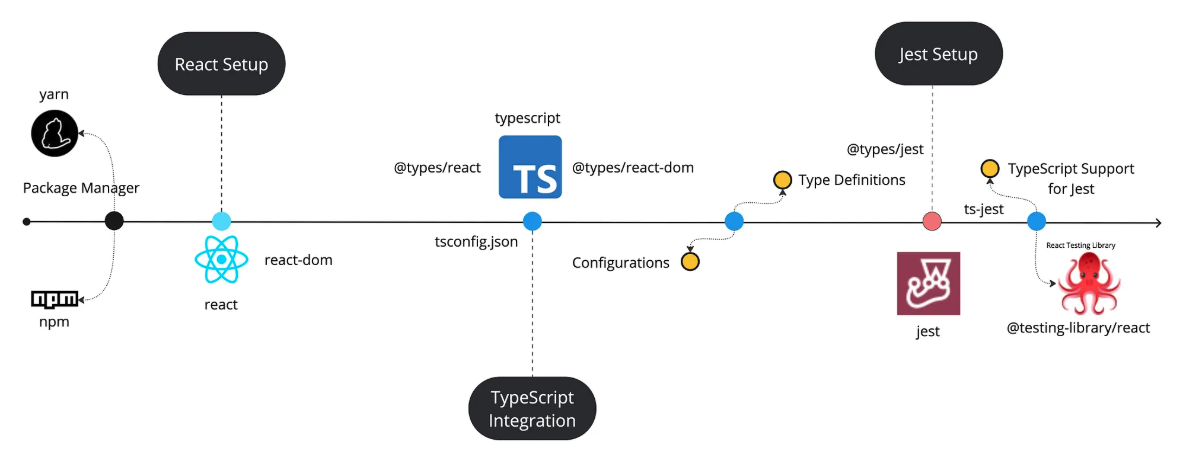
\includegraphics[scale=0.3]{jest.png}
      \caption{The Expo Jest React Native Testing Setup\cite{LevelUp2025}}
      \label{figure:jest}
    \end{center}
  \end{figure}
  
Jest (A JavaScript Testing Framework that works with React Native and Expo) was also used to make unit tests to validate whether components render and if they render correctly. The use of Jest was made even easier as Jest comes pre setup with a react native expo project so minimal setup is required and there is copious documentation for reference while developing. Jest tests were written in the components/tests/ directory in typescript to ensure strong type checking while validating the app. A common test is to be able to render a component and check if it is the correct component. This is done by using the toBeTruthy() method to check if the component is rendered correctly. The tests were run using the command line and the results were checked to ensure that all tests passed.
 % Add one file per section.
\clearpage

\section{Results \& Evaluation}\label{results}

% Results are often presented in tables, figures and other relevant illustrations. Include text that refers to these figures/tables. 

\subsection{Evaluation Process}
For the first round of app evaluation, 5 users who were women between the ages of 30 and 65 were recruited to watch a demo video of the app and fill out a SUS and a few long answer questions with their feedback. These participants were recruited via email and were asked to read through a participant information sheet before participating.

\begin{table}[h!!]
    \begin{tabular}{ll}
    \hline
    SUS Scores(n=5) &      \\ \hline
                    & 67.5 \\
                    & 85   \\
                    & 72.5 \\
                    & 77.5 \\
                    & 65   \\
        Average Score & 73.5
    \end{tabular}
    \end{table}

%% Susan: 
%% its > it's 
From the average SUS score of 73.5, it is clear that the app is usable as its in the top 27\% of scores, but it could be improved.

%% Susan: 
%% included more instructions > more instructions were included
After obtaining these results, changes were made to the app's look and feel and included more instructions. AB Testing was then conducted with more participants to see if the changes made had a positive impact on the SUS score. 

**Will put results here** 

The app was then rated according to the MARS rating system and compared to the other app rated at the beginning of the study. **Results here** 

\subsection{Results of Evaluation}
This Section includes a direct interpretation of the gathered data and evaluation processes. 

 
\clearpage
\section{Discussion \& Reflection}

\subsection{Interpreting the Results}

Here you will discuss your findings. This is especially relevant for research projects. You might 
 interpret what the data and evaluation implies, both for future research and for practice (if appropriate). 
 
 The discussion is \textbf{not} a review of literature. You should try to compare research findings with previous work,
provide  explanations for your findings,
discuss  research findings, in terms of their contribution.

The initial research shows many women prefer to write down their symptoms manually instead of using an app, but were hesitant to specify why. 

While this may be a helpful symptom tracking app to show data to your doctor, this will not make a big impact on the overall knowledge and awareness of peri-menopause and the struggle that perimenopausal women go through during this transition. Better education in school about menopause and perimenopause along with mandatory and detailed education for doctors would be a better and more effective solution to the problem.

\subsection{Reflection}
Trying different implementation strategies, while worthwhile, meant much time was wasted switching between different languages and frameworks. This was a valuable learning experience, but it did slow down the project. Future projects should have a more clear implementation plan from the start to avoid this issue.

\subsection{Challenges}
Version control practices became lax at one point during the project which had repercussions on the project timeline. Future projects should have a more strict version control policy. 

\subsection{Limitations}
A small number of participants did make the data collected less reliable. The app was also not fully tested on all devices and platforms, so there may be some bugs or inconsistencies that were not caught.


\subsection{Future Work}
Transitioning the application to use only typescript instead of a combination of typescript and javascript would be a good next step. This would allow for more strict type checking and reduce runtime errors. While researching, many good points were discovered about Expo router instead of React Navigation. While React Navigation did not pose and major issues and was easy to use, Expo Router may prove to be more sustainble for long term development and should be considered. More analysis data should be added to the analysis page to provide the user with possible triggers or which symptos are commonly tracked together or to notify the user when an unusual pattern is detected. Additionally, the app could be expanded to include more features such as a community forum where users can share their experiences and advice with each other. The app could be expanded to include more customization options for users, such as the ability to change the color scheme or font size. The app could also be expanded to include more detailed analysis of user data, such as predicting when a user's next period will start based on their previous data, or include a quiz to indicate what stage of menopause they may be in and why. Finally, the app could be expanded to include more educational resources on perimenopause and related topics, such as articles, videos, and podcasts. A database connection could also be added so that those who want to back up their data can do so. Integrating the app with Apple Health or health watches and other apps to reduce the amount of work a user has to go through to input data may make the app more popular and give the app more data to increase analysis accuracy. Creating compatibility with the NHS digital front door app that is currently in the works would also be a good next step to increase the app's reach and usability. This could be accomplished in the form of easy data exporting from the tracking app to the NHS app so doctors are more aware of what their patients are going through and are better equipped to help perimenopausal individuals.

 
\clearpage
\section{Conclusion}\label{conc}

By interpreting the results of this study, it was shown that there is a gap in the market for private and discreet focused period and symptom tracking apps. By creating a usable app with real data privacy and anonymity the aim and goals of this study have been accomplished. The app has evolved and improved with each round of user review and feedback which is reinforced by the rating scores and statists collected. Research showed that many women prefer to track symptoms manually but from the background research it is a likely possibility that this is due to lack of privacy and the sensitivity of data collected. It also may likely be due to cultural attitudes that do not encourage this sort of information to be discussed and reviewed.



%--------------------------------
% Bibliography
%--------------------------------
\clearpage
\setstretch{1.0}  % 1.0 line spacing. 
\bibliographystyle{abbrv}
\bibliography{bibliography}
% add references to the file called bibliography.bib
\clearpage

%--------------------------------
% Appendices
%--------------------------------
\appendix
\setstretch{1.5} % 1.5 line spacing.
\section{Appendix}

This is where you can include your documentation.

Remember that the marker is not required to read this, but might well check to ensure that you have included product documentation, and ethical approval, as required.
\subsection{Tests}
The following are all the aspects of the app that the JEST tests cover.
\begin{itemize}
  \item The Analysis component renders correctly with default settings
  \item The Analysis component renders without errors
  \item Verifies that the element with the test ID analysis-container is present in the rendered output of the Analysis Screen component
  \item Ensures the Calendar component renders without errors
  \item Verifies that the Calendar component is displayed correctly with the current month and year
  \item Navigates to the previous month when the left button (<) is pressed in the Aalendar component
  \item Navigates to the next month when the right button (>) is pressed in the Aalendar component
  \item Ensures the Home component renders without errors
  \item Verifies that the text ``Symptoms'' and ``Period'' are present in the rendered output
  \item Ensures the Learn component renders without errors
  \item Verifies that the tab buttons ``For You'' ``Recent'' ``Symptom Relief'' and ``All Articles'' are displayed
  \item Verifies that the Recent tab's font weight changes to bolder indicating it is selected
  \item Correctly filters articles based on the ``symptoms'' keyword
  \item Opens the article URL when an article is pressed
  \item Ensures the MostCommon component renders without errors
  \item Verifies that all common symptoms are displayed with their corresponding severity levels
  \item Ensures the PeriodSquare component renders without errors
  \item Checks that the text style includes fontSize: 15 and color: ``\#009668''
  \item Checks that the text style includes color: 'white' when selected
  \item Ensures the Slider component renders without errors
  \item Renders the Slider component correctly with large text enabled
  \item Ensures the Slider component renders correctly when the highContrast setting is enabled
  \item Renders the Slider component correctly with a specific value
  \item Ensures the TabButton component renders without errors
  \item Renders the Track component correctly
  \item Updates selected period state when a period button is pressed
  \item Saves data when the save button is pressed
  \item Ensures the TwoWeek component renders without errors
  \item Verifies that the element with the test ID date-range is present in the rendered output
\end{itemize}

\subsection{Ethical Approval Form}
\includepdf[pages=-,scale=0.9]{Ethics_form.pdf}
\begin{figure}[h!!]
    \begin{center}
      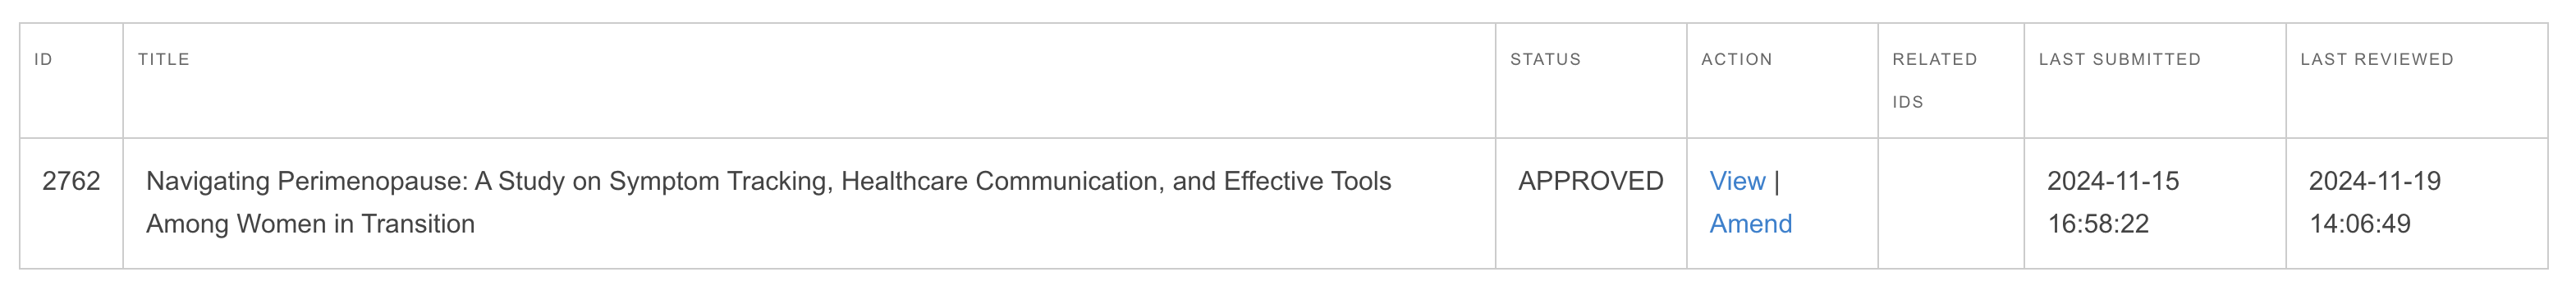
\includegraphics[scale=0.3]{EthicsApproval.png}
      \caption{Ethics Approval.}
      \label{figure:ethics-approval}
    \end{center}
  \end{figure}
  
\subsection{Participant Information Sheet }
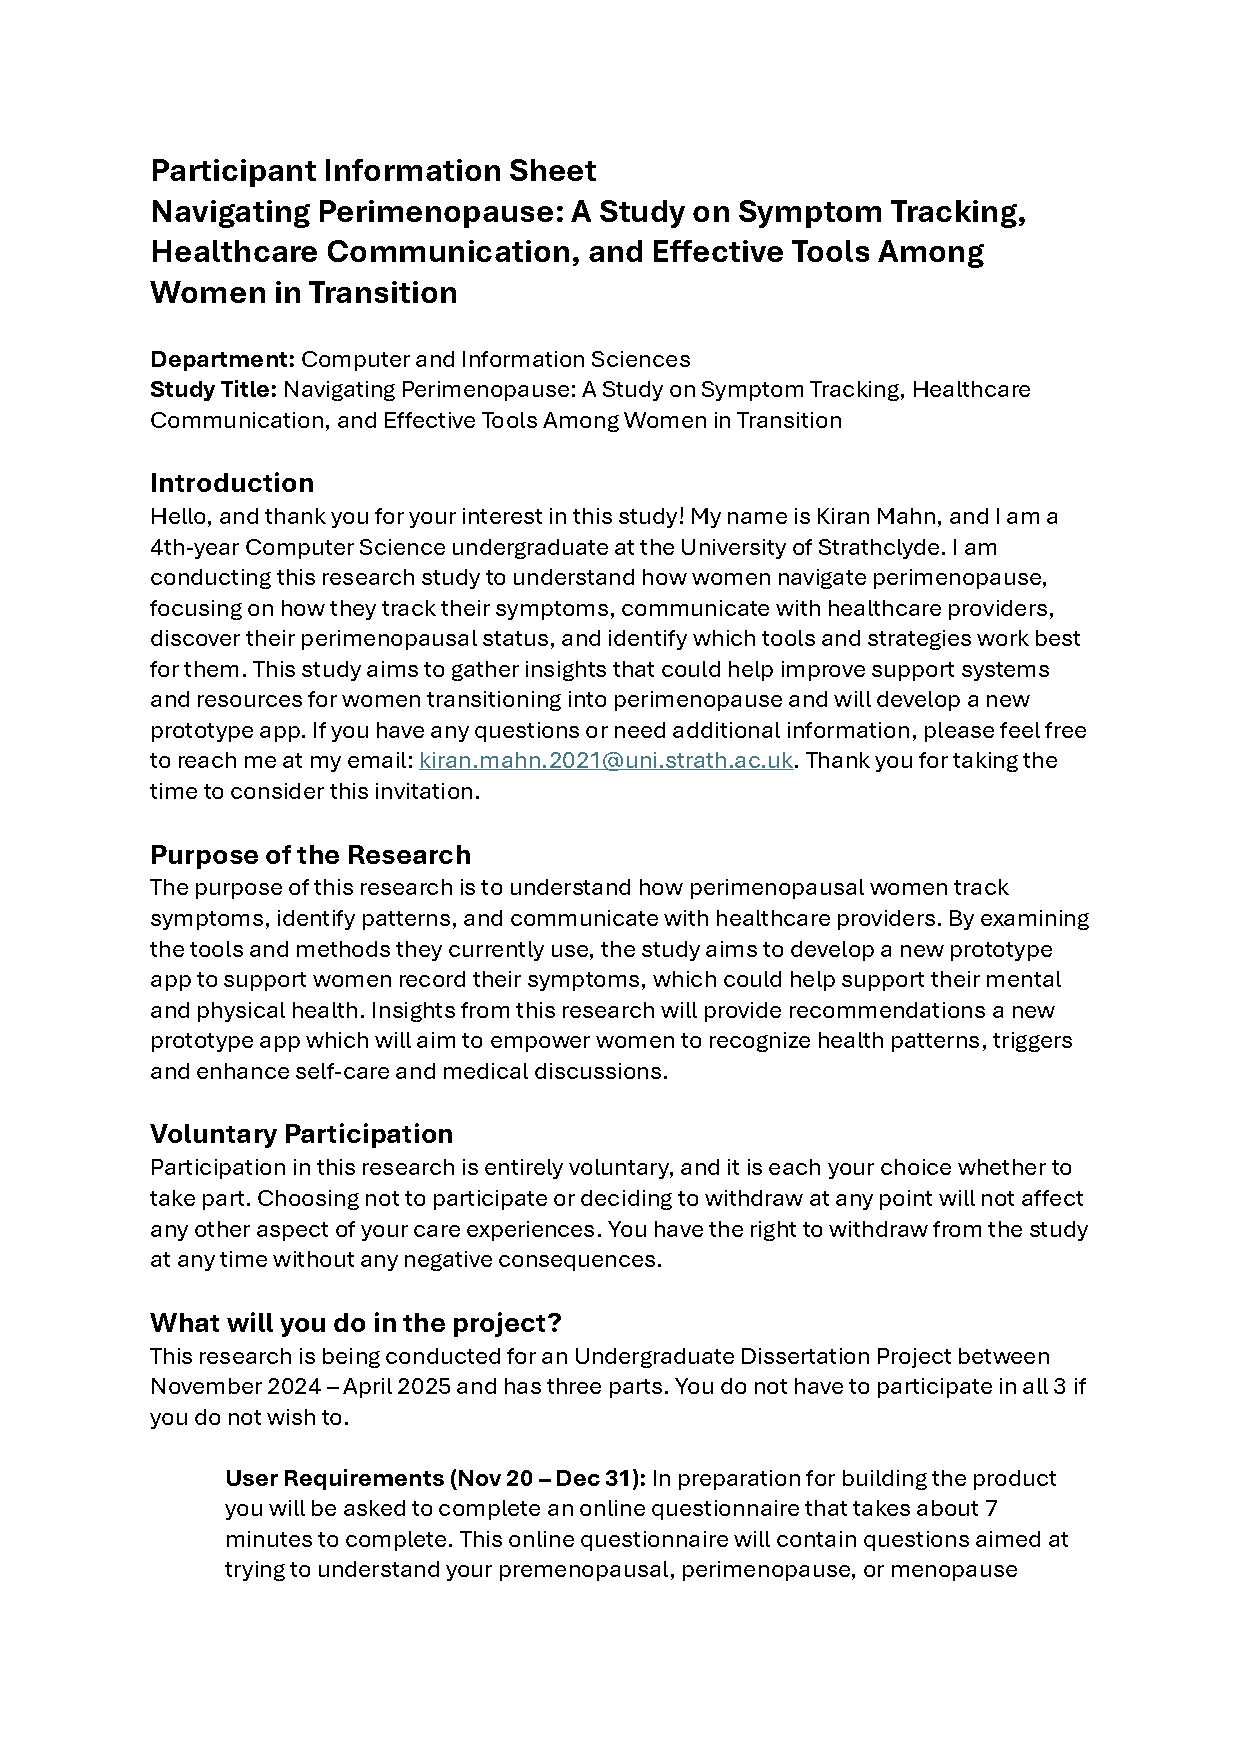
\includepdf[pages=-,scale=0.9]{Participant_Information_Sheet.pdf}

\subsection{Consent Form }
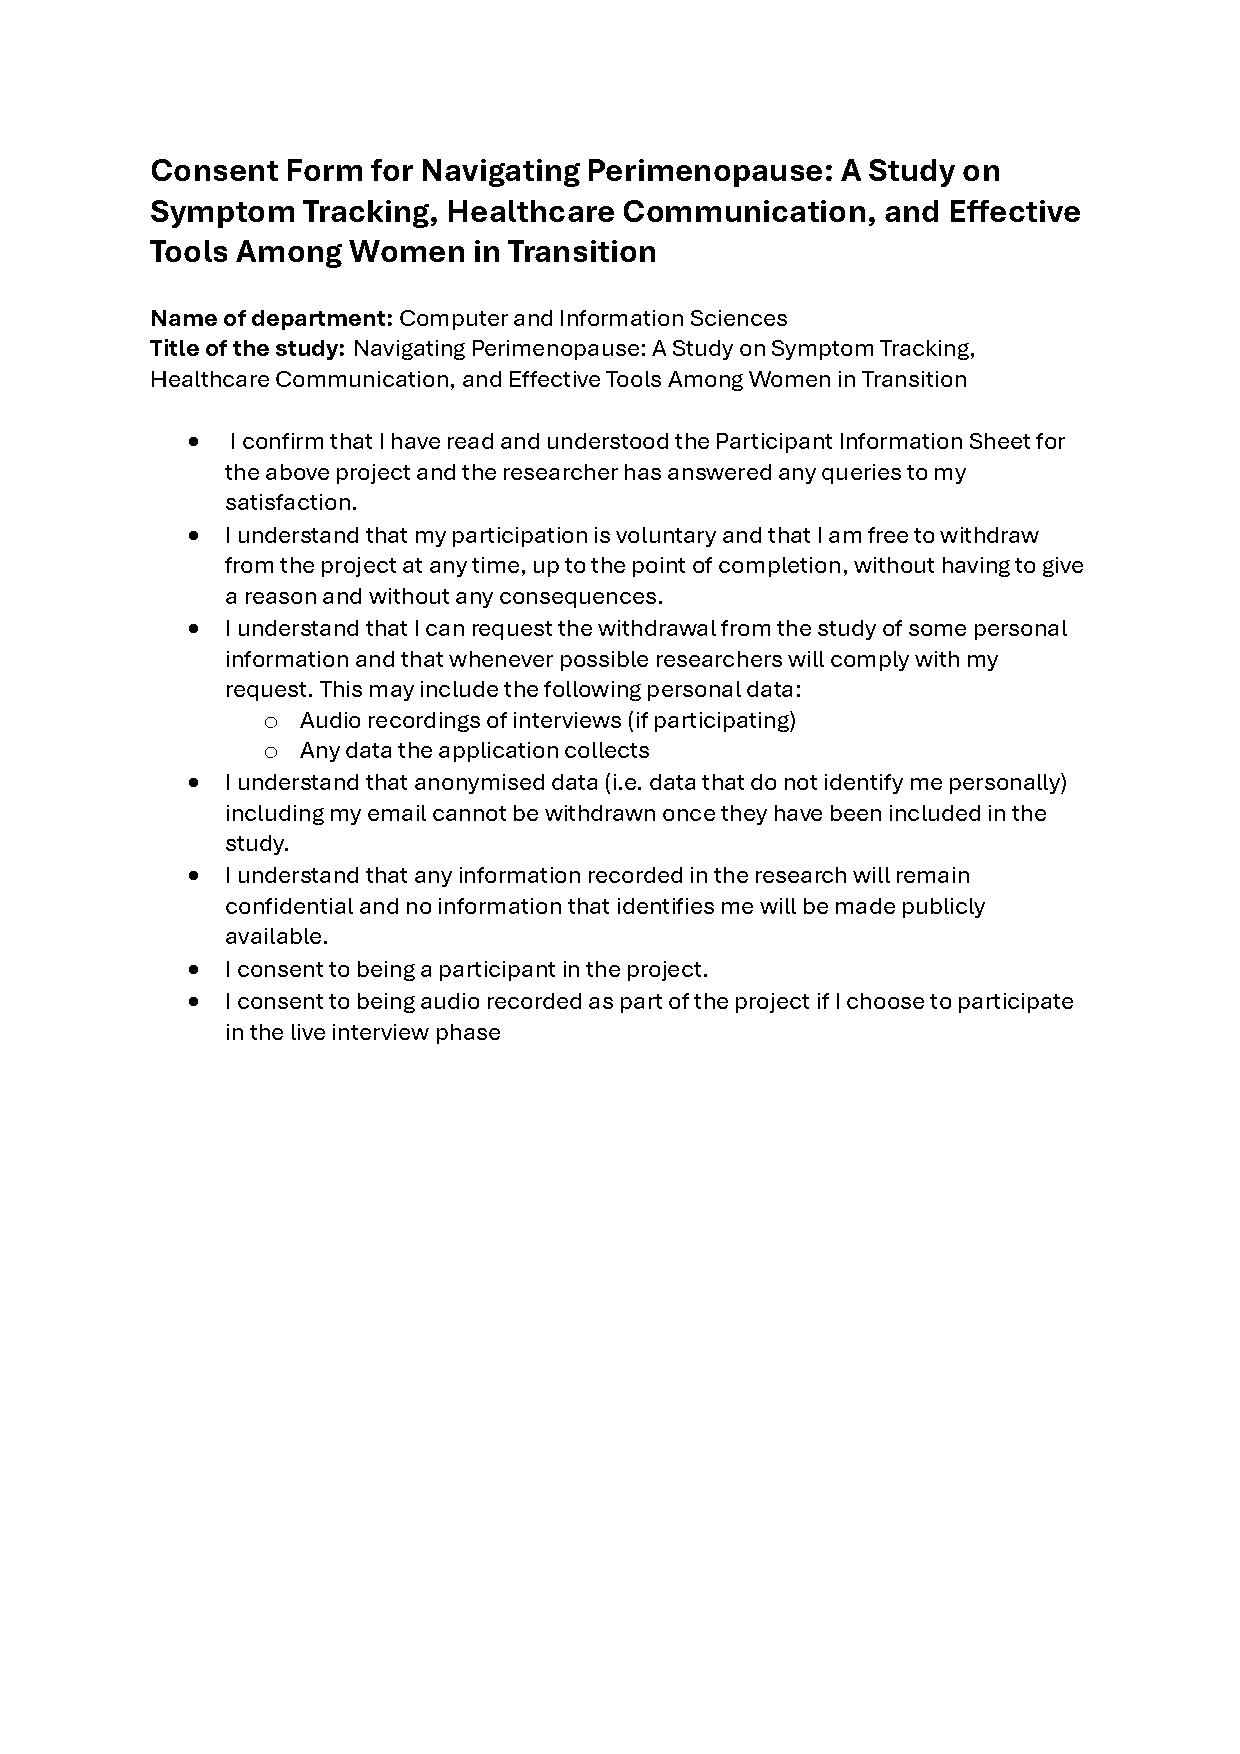
\includepdf[pages=-,scale=0.9]{Consent_Form.pdf}

\subsection{MARS Reviews}
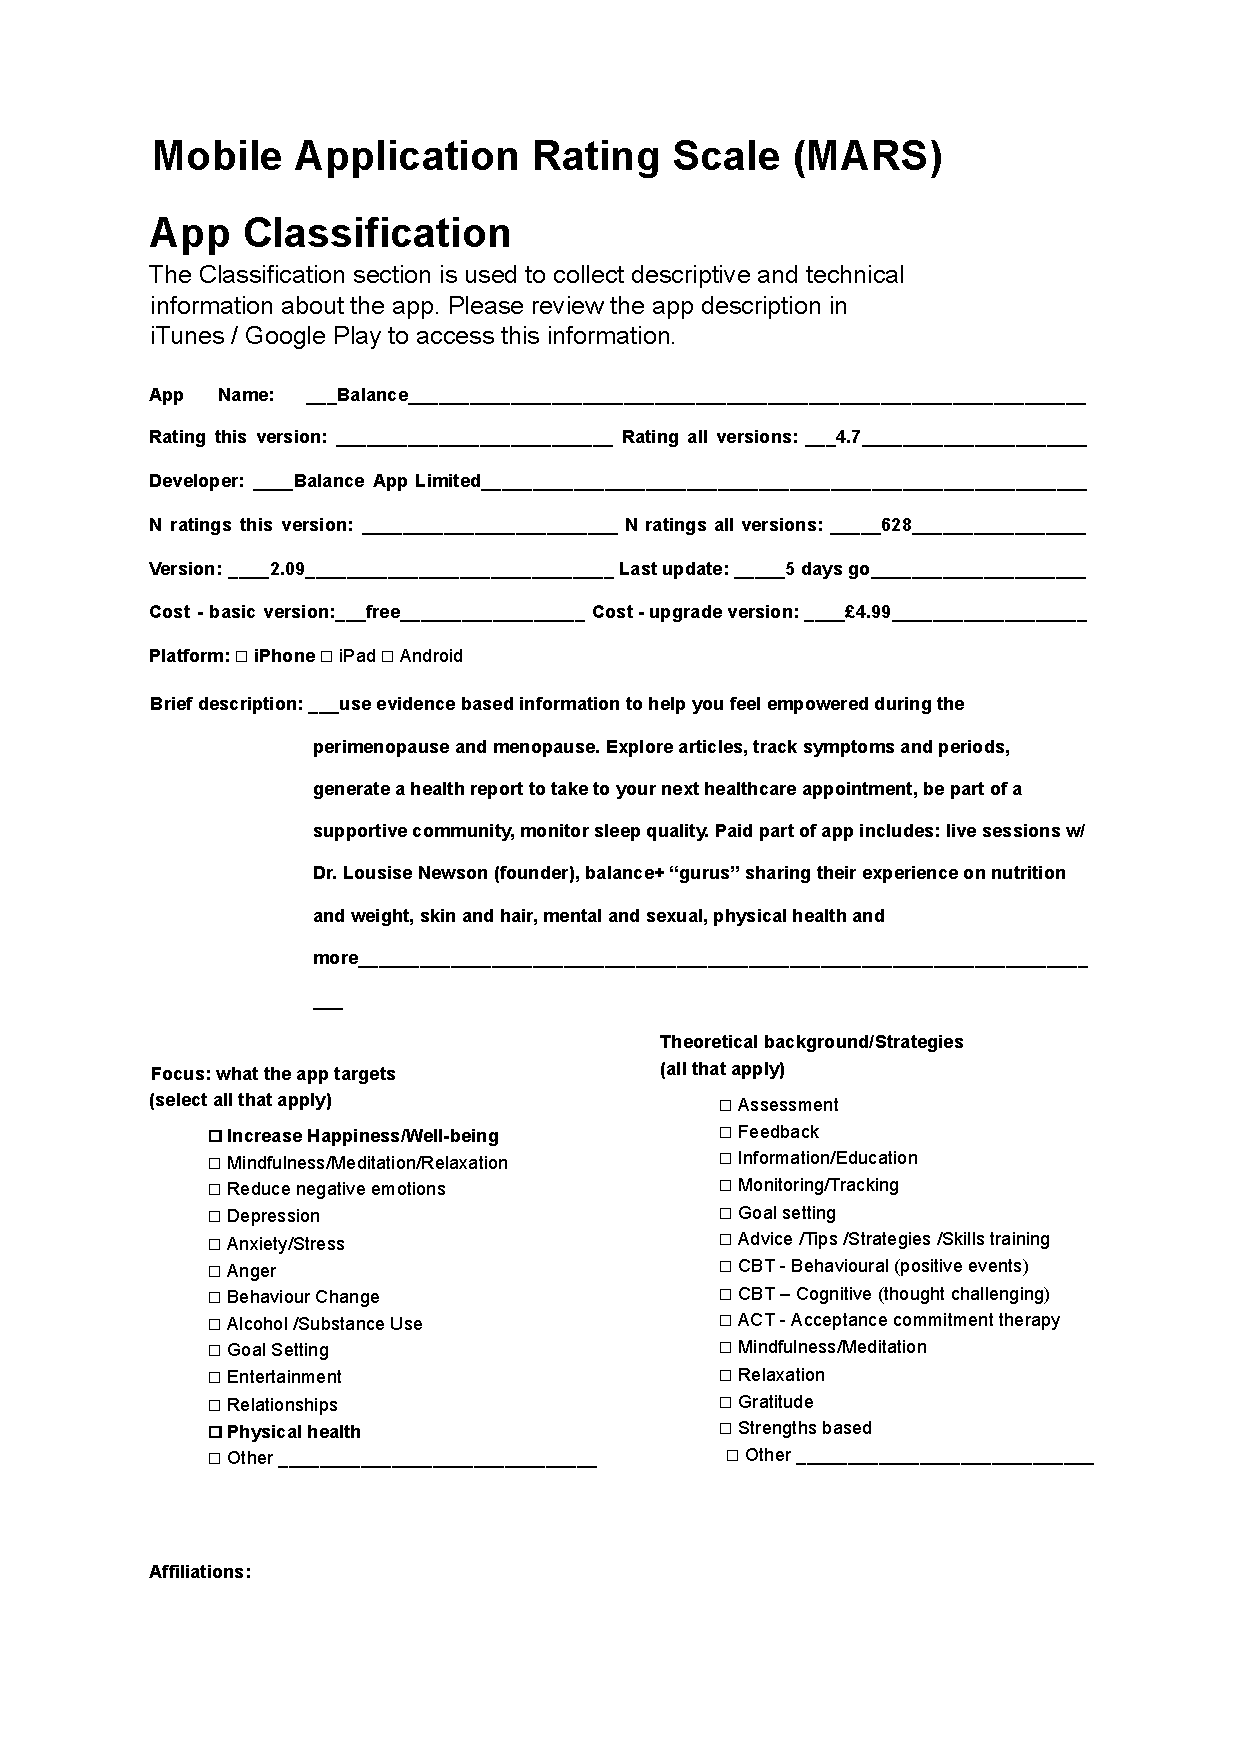
\includepdf[pages=-,scale=0.9]{Balance.pdf}
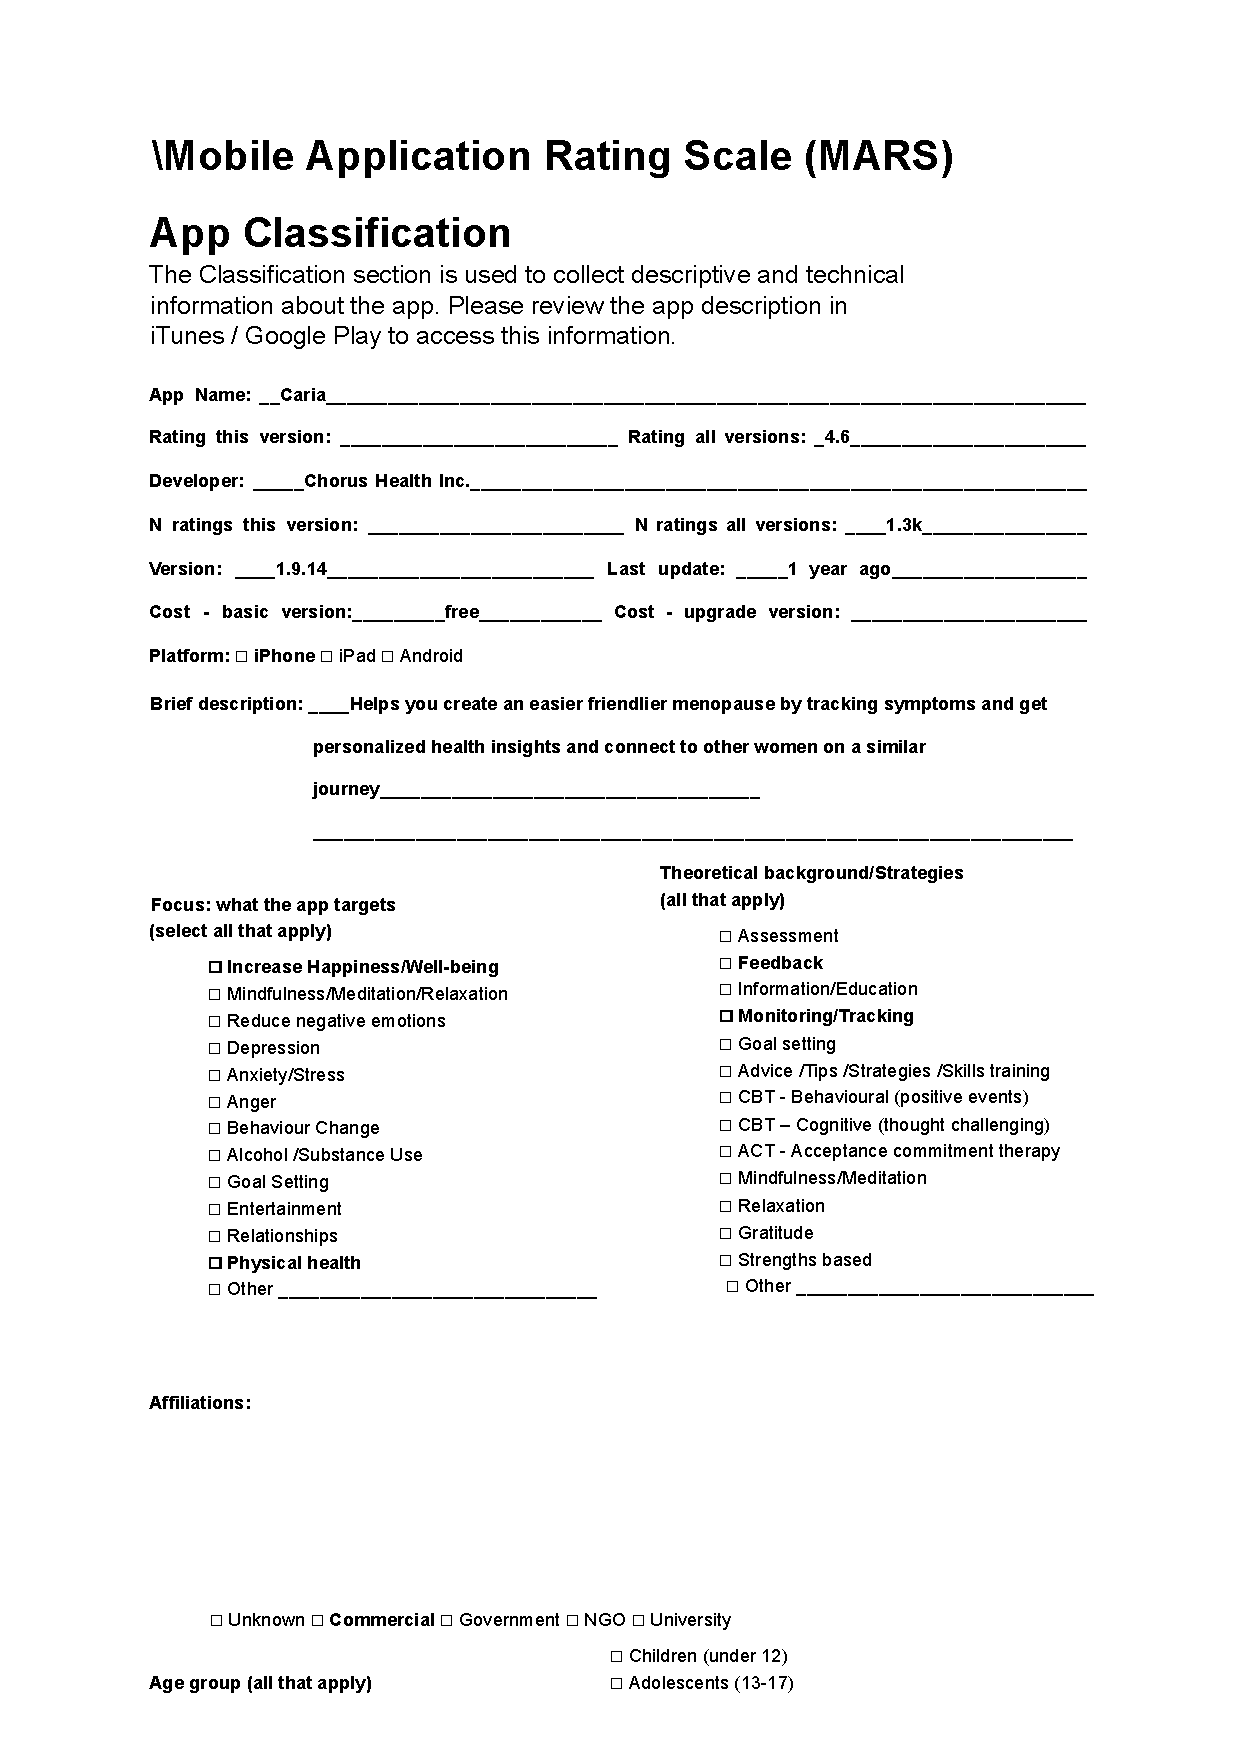
\includepdf[pages=-,scale=0.9]{Caria.pdf}
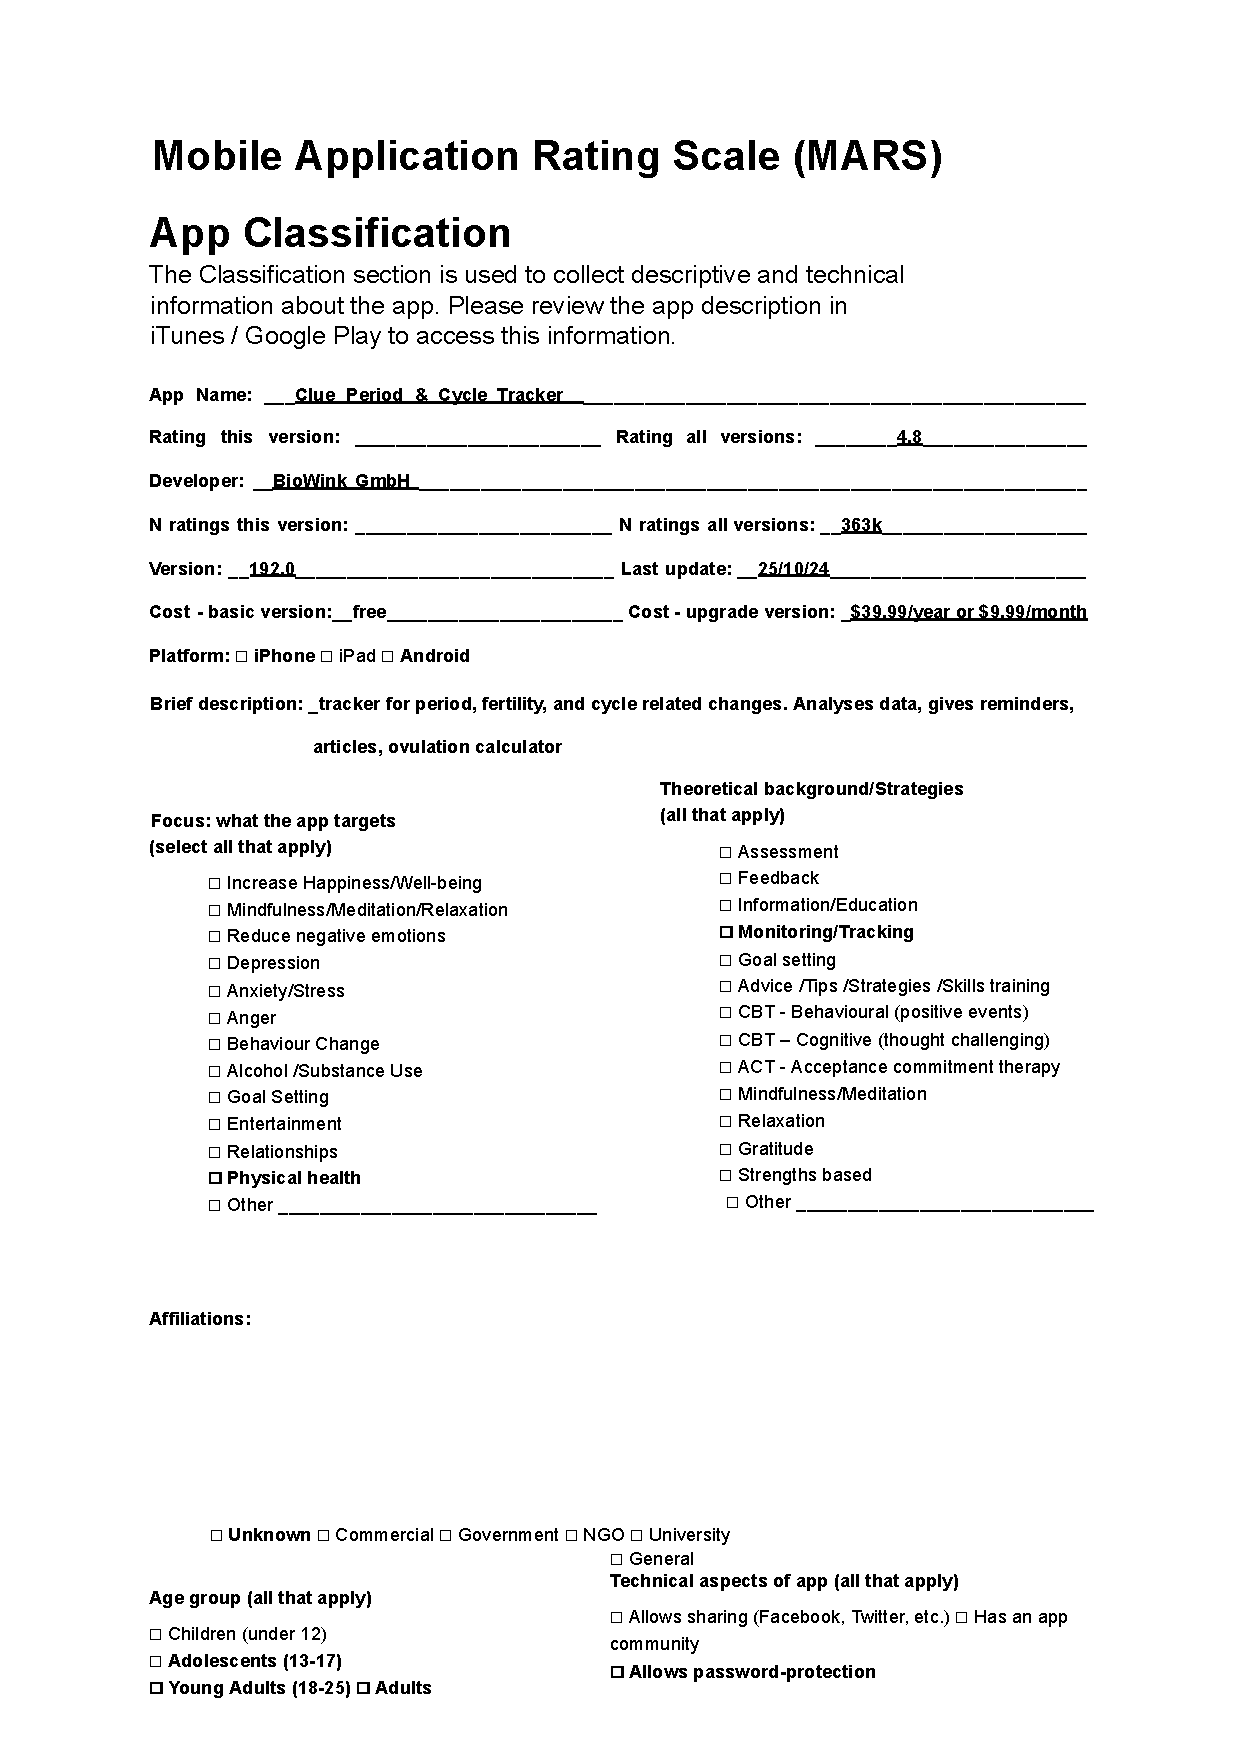
\includepdf[pages=-,scale=0.9]{Clue.pdf}
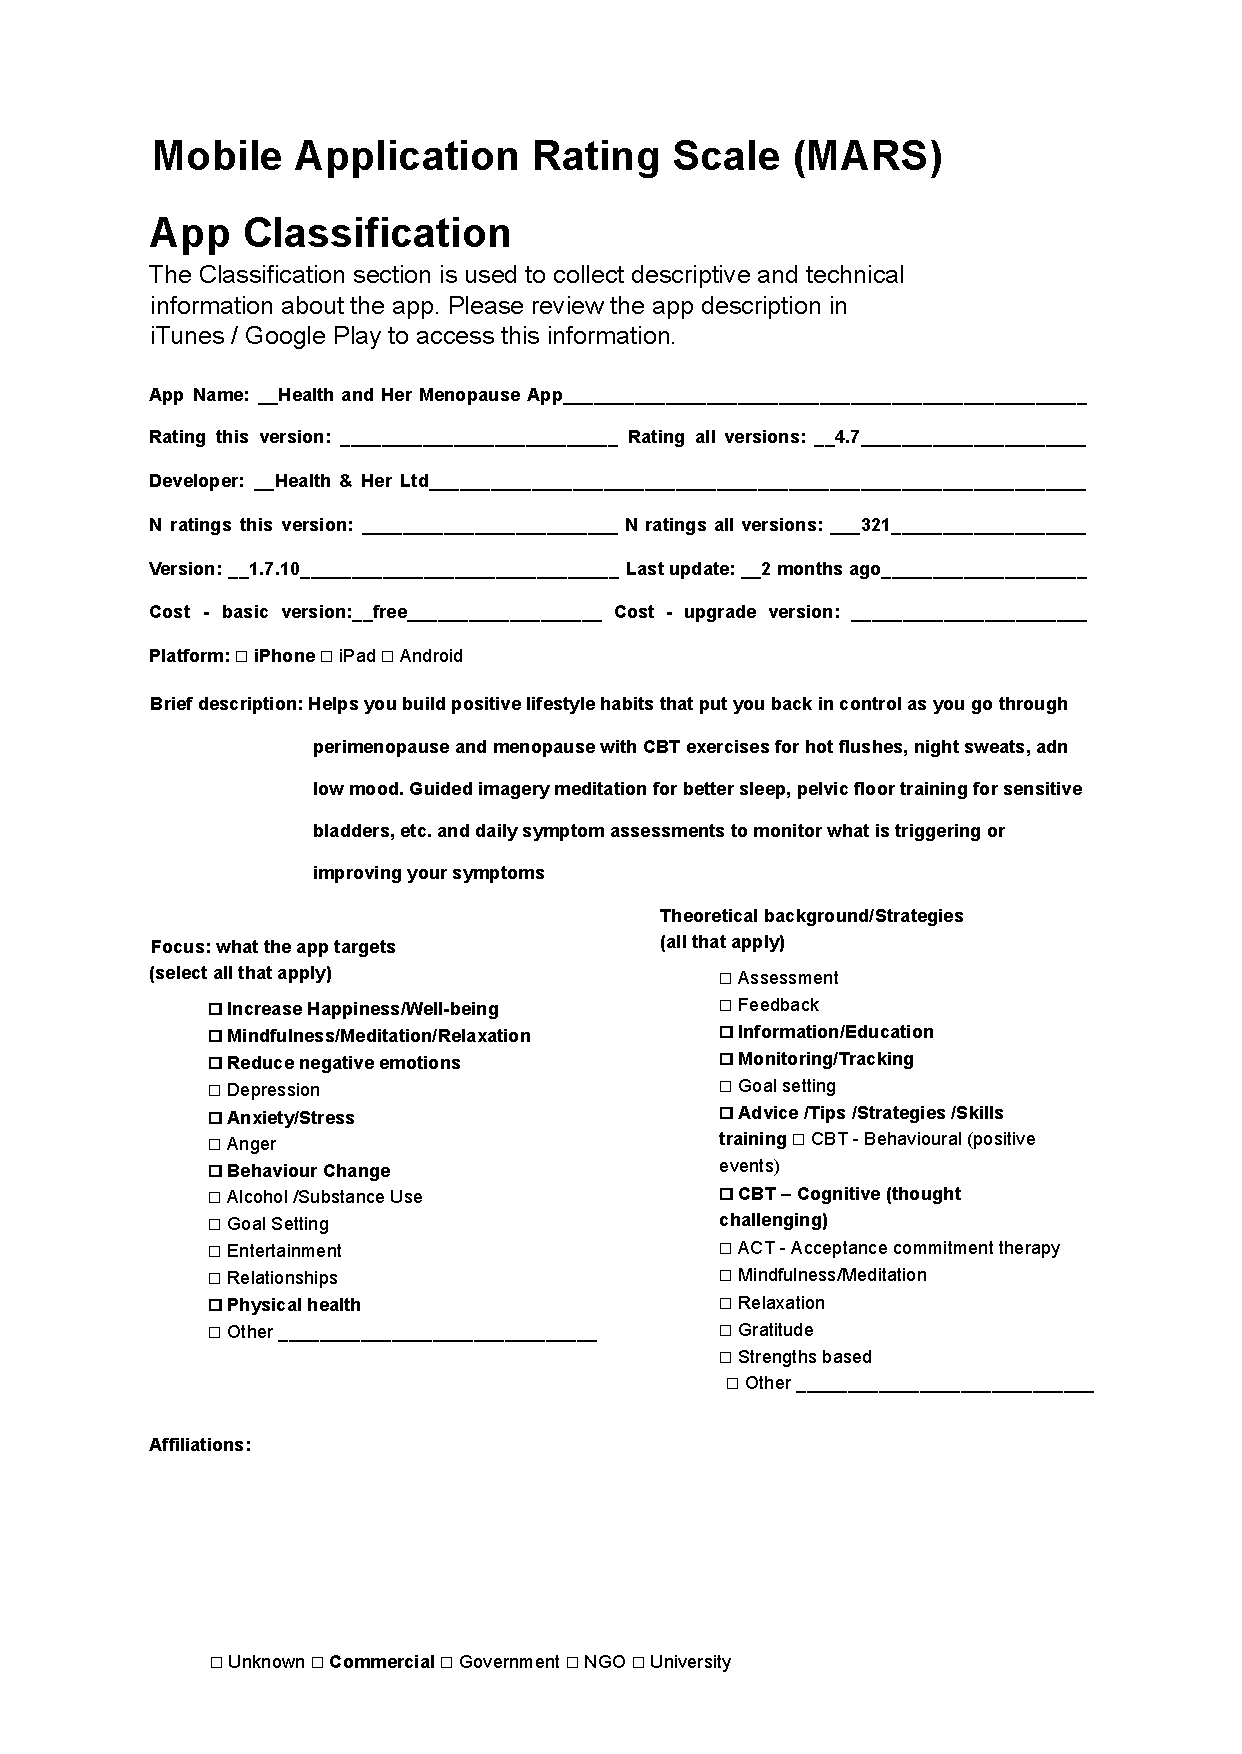
\includepdf[pages=-,scale=0.9]{HealthandHer.pdf}
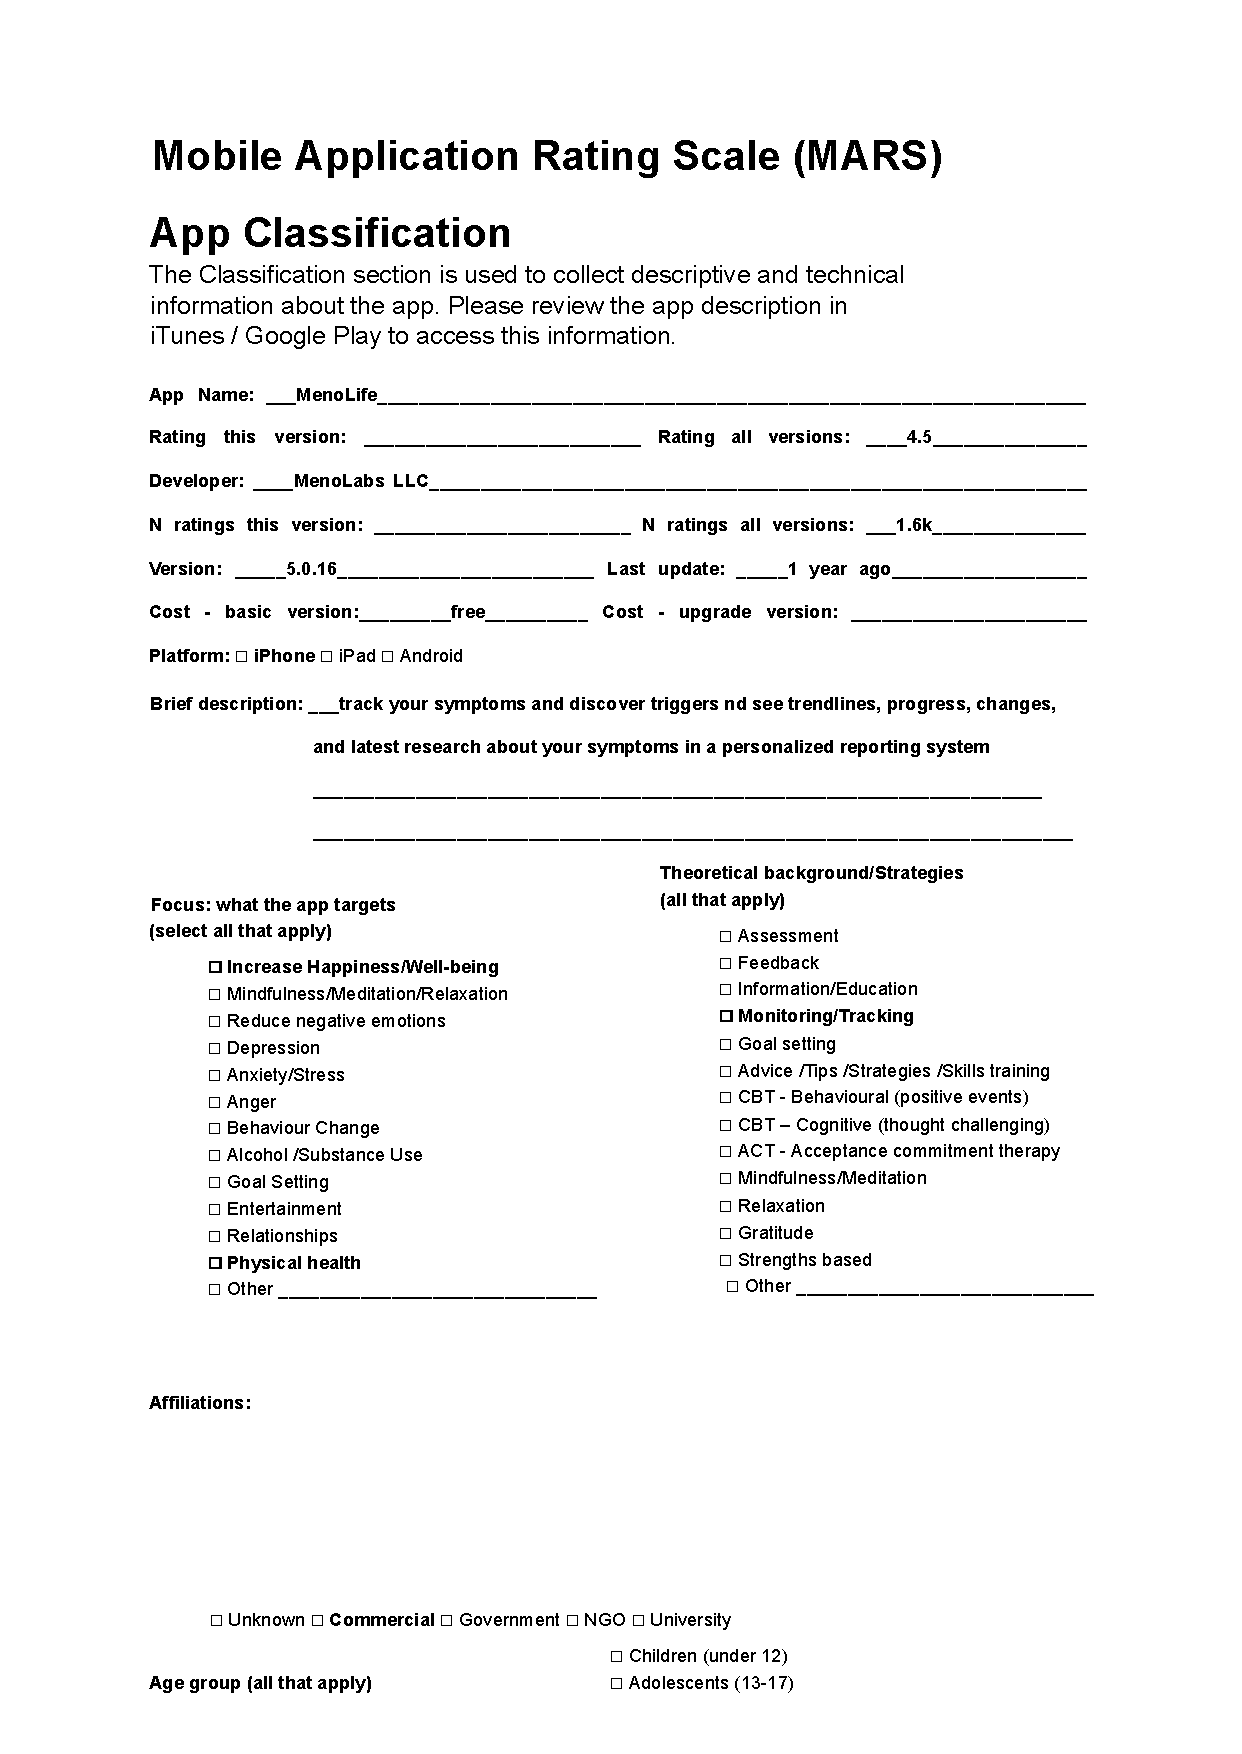
\includepdf[pages=-,scale=0.9]{MenoLife.pdf}
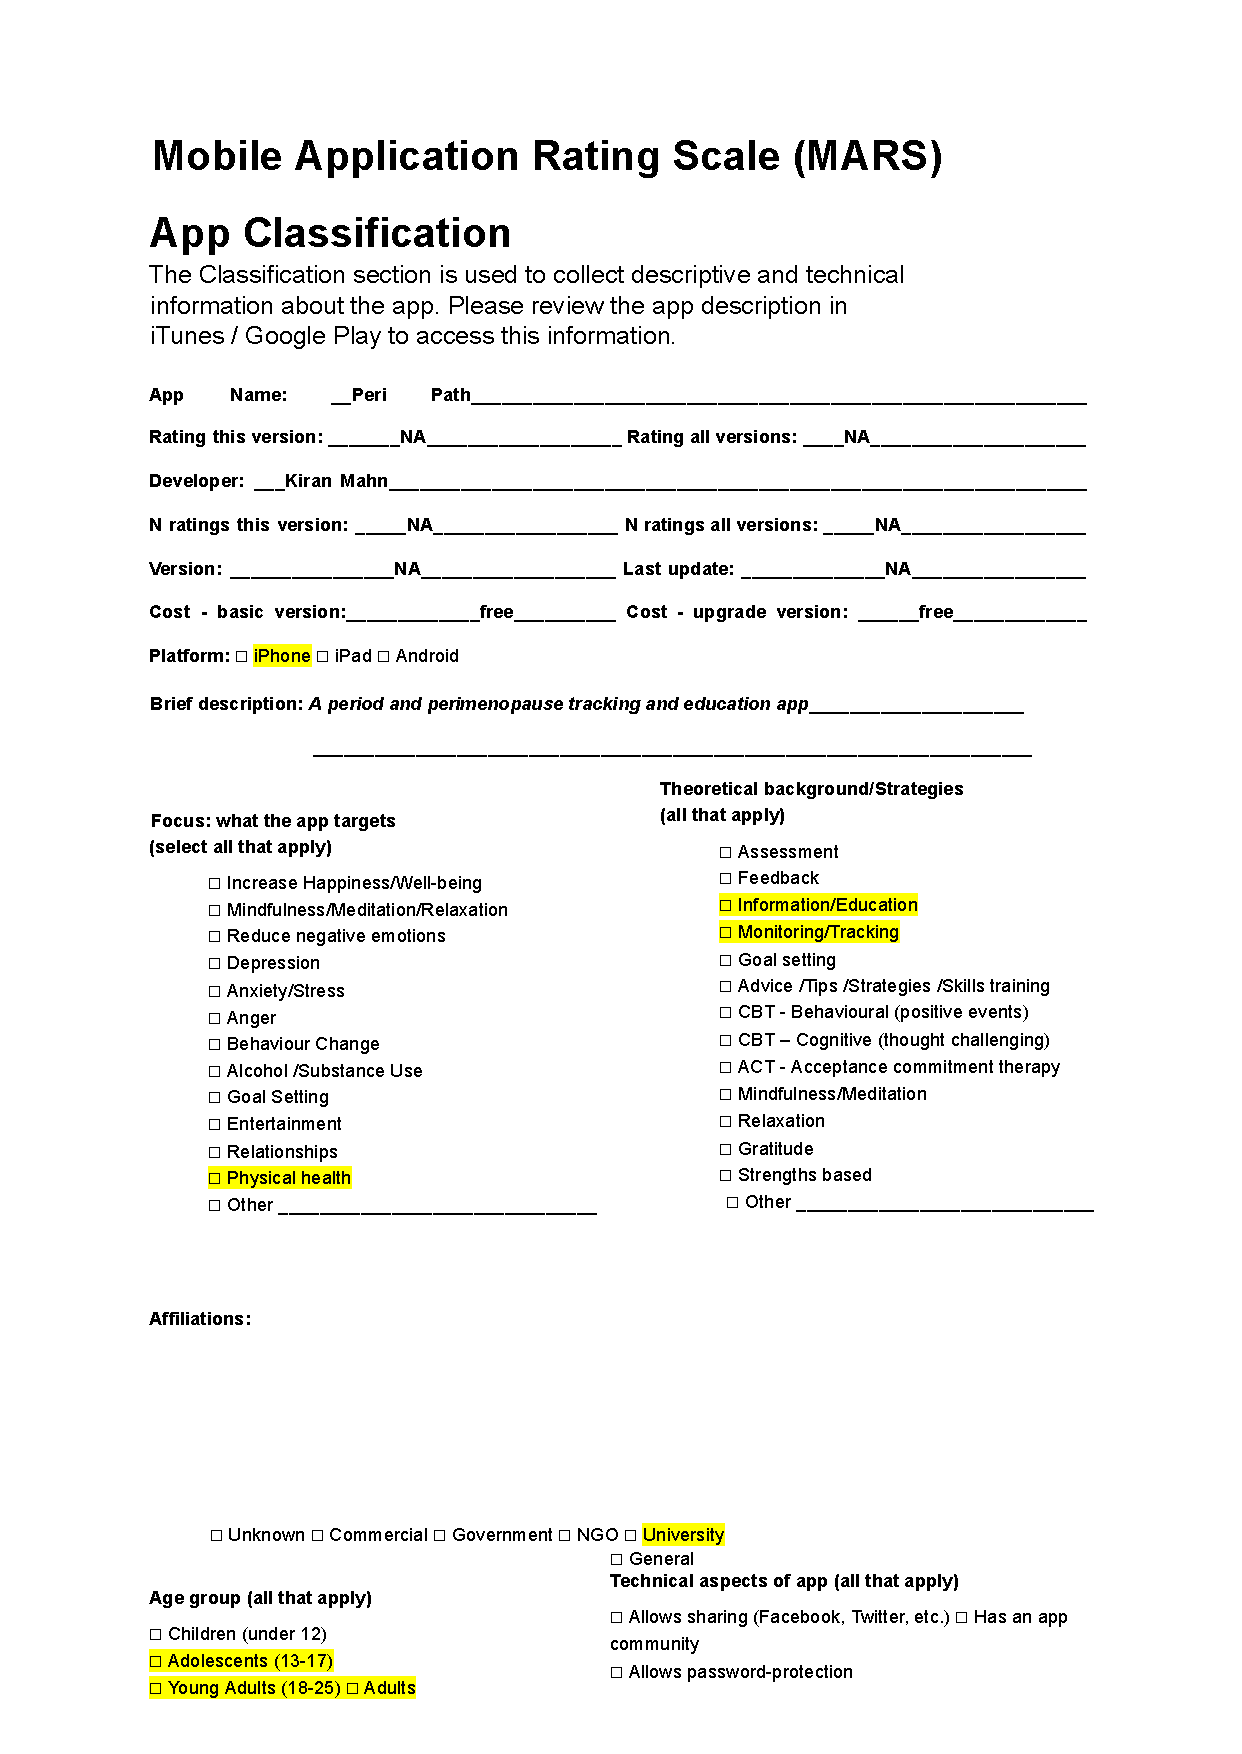
\includepdf[pages=-,scale=0.9]{PeriPath.pdf}
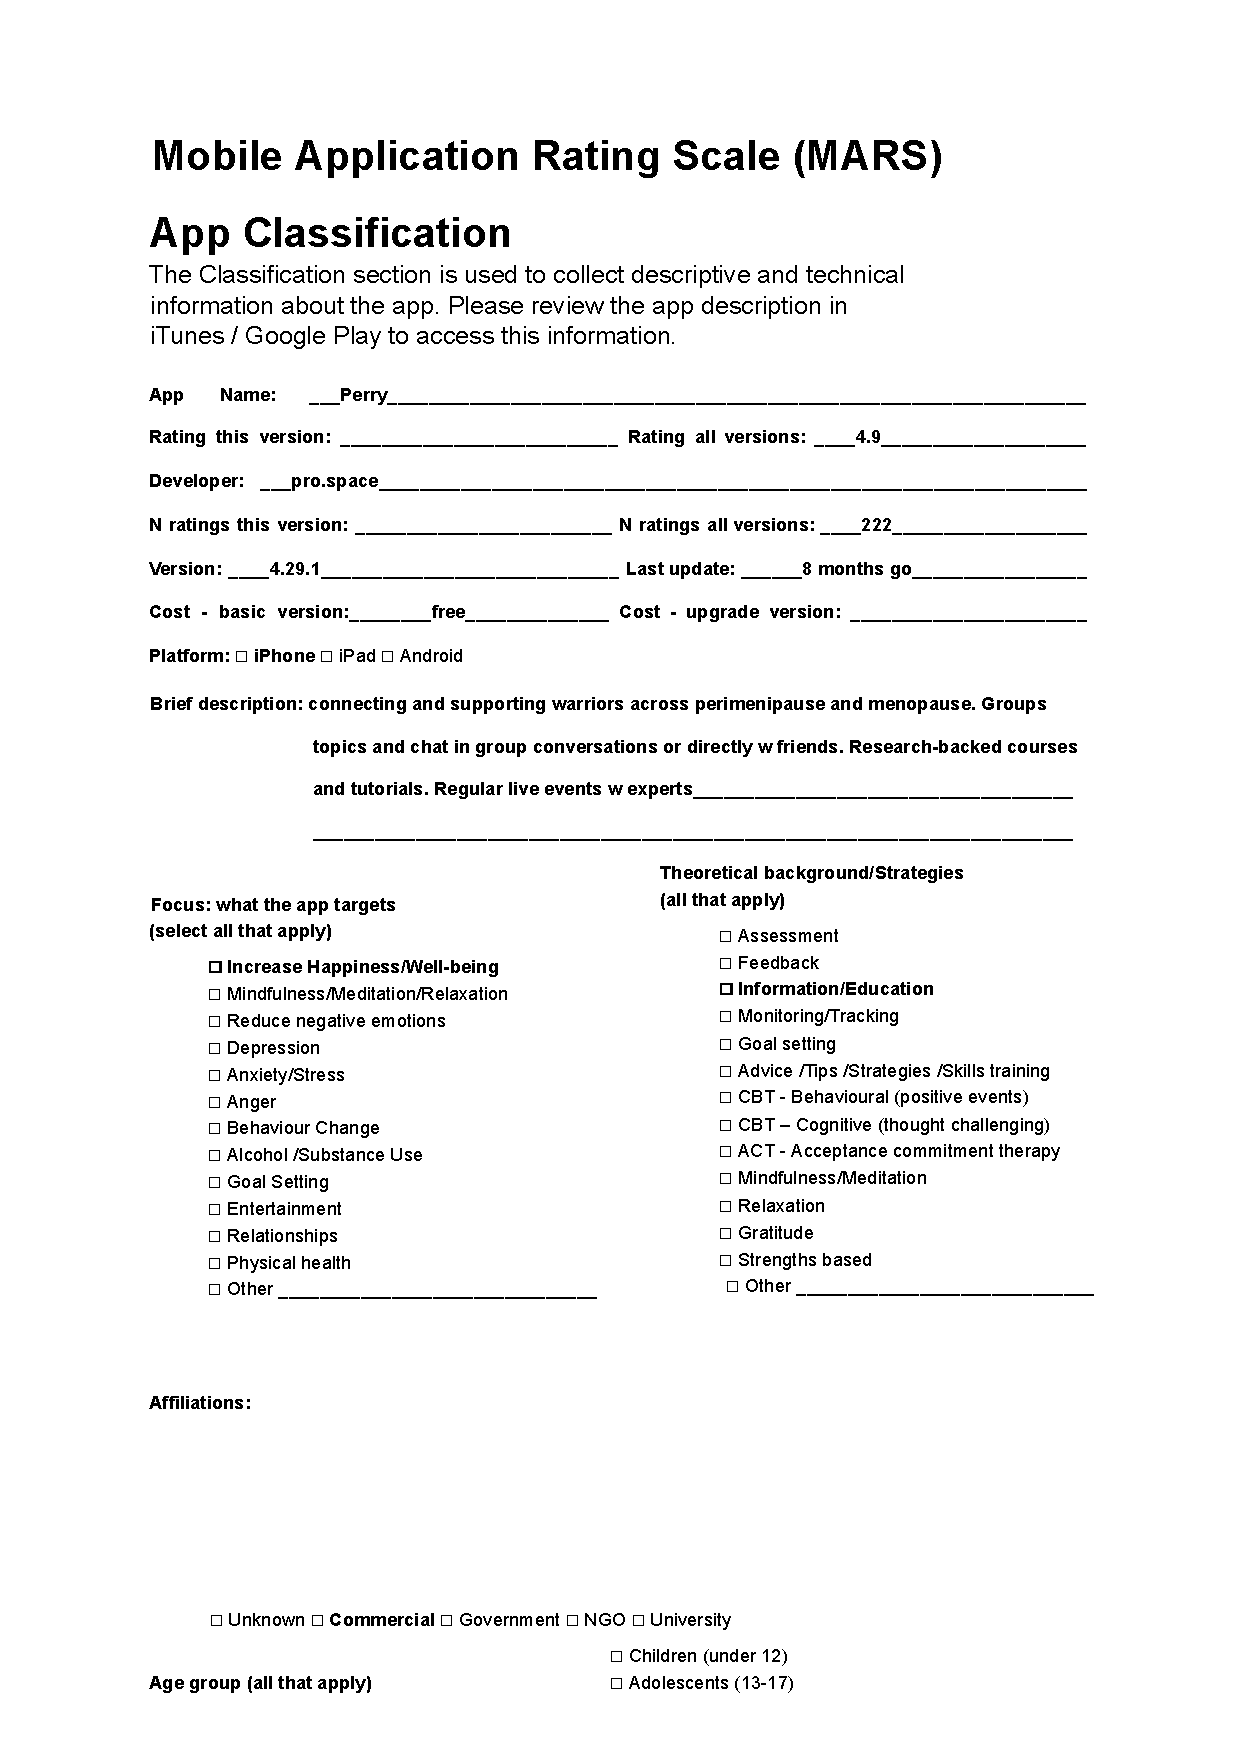
\includepdf[pages=-,scale=0.9]{Perry.pdf}
\includepdf[pages=-,scale=0.9]{OtherMARSEvals.pdf}
\clearpage


 

 % Add one file per appendix

\end{document}
